\hypertarget{Predict_8c}{
\section{Predict.c File Reference}
\label{Predict_8c}\index{Predict.c@{Predict.c}}
}
{\tt \#include \char`\"{}party.h\char`\"{}}\par


Include dependency graph for Predict.c:\begin{figure}[H]
\begin{center}
\leavevmode
\includegraphics[width=159pt]{Predict_8c__incl}
\end{center}
\end{figure}
\subsection*{Functions}
\begin{CompactItemize}
\item 
void \hyperlink{Predict_8c_a0}{C\_\-splitnode} (SEXP node, SEXP learnsample, SEXP control)
\item 
SEXP \hyperlink{Predict_8c_a1}{C\_\-get\_\-node} (SEXP subtree, SEXP newinputs, double mincriterion, int numobs)
\item 
SEXP \hyperlink{Predict_8c_a2}{R\_\-get\_\-node} (SEXP subtree, SEXP newinputs, SEXP mincriterion, SEXP numobs)
\item 
SEXP \hyperlink{Predict_8c_a3}{C\_\-get\_\-nodebynum} (SEXP subtree, int nodenum)
\item 
SEXP \hyperlink{Predict_8c_a4}{R\_\-get\_\-nodebynum} (SEXP subtree, SEXP nodenum)
\item 
SEXP \hyperlink{Predict_8c_a5}{C\_\-get\_\-prediction} (SEXP subtree, SEXP newinputs, double mincriterion, int numobs)
\item 
SEXP \hyperlink{Predict_8c_a6}{C\_\-get\_\-nodeweights} (SEXP subtree, SEXP newinputs, double mincriterion, int numobs)
\item 
int \hyperlink{Predict_8c_a7}{C\_\-get\_\-node\-ID} (SEXP subtree, SEXP newinputs, double mincriterion, int numobs)
\item 
SEXP \hyperlink{Predict_8c_a8}{R\_\-get\_\-node\-ID} (SEXP tree, SEXP newinputs, SEXP mincriterion)
\item 
void \hyperlink{Predict_8c_a9}{C\_\-predict} (SEXP tree, SEXP newinputs, double mincriterion, SEXP ans)
\item 
SEXP \hyperlink{Predict_8c_a10}{R\_\-predict} (SEXP tree, SEXP newinputs, SEXP mincriterion)
\item 
void \hyperlink{Predict_8c_a11}{C\_\-getpredictions} (SEXP tree, SEXP where, SEXP ans)
\item 
SEXP \hyperlink{Predict_8c_a12}{R\_\-getpredictions} (SEXP tree, SEXP where)
\item 
void \hyperlink{Predict_8c_a13}{C\_\-getweights} (SEXP tree, SEXP where, SEXP ans)
\item 
SEXP \hyperlink{Predict_8c_a14}{R\_\-getweights} (SEXP tree, SEXP where)
\item 
void \hyperlink{Predict_8c_a15}{C\_\-weights} (SEXP tree, SEXP newinputs, double mincriterion, SEXP ans)
\item 
SEXP \hyperlink{Predict_8c_a16}{R\_\-weights} (SEXP tree, SEXP newinputs, SEXP mincriterion)
\item 
SEXP \hyperlink{Predict_8c_a17}{R\_\-predict\-RF} (SEXP forest, SEXP newinputs, SEXP mincriterion, SEXP oobpred)
\item 
SEXP \hyperlink{Predict_8c_a18}{R\_\-predict\-RF2} (SEXP forest, SEXP response, SEXP newinputs, SEXP mincriterion, SEXP oobpred)
\item 
SEXP \hyperlink{Predict_8c_a19}{R\_\-predict\-RF\_\-weights} (SEXP forest, SEXP newinputs, SEXP mincriterion, SEXP oobpred)
\end{CompactItemize}


\subsection{Detailed Description}
Node splitting and prediction

\begin{Desc}
\item[Author:]\begin{Desc}
\item[Author]hothorn \end{Desc}
\end{Desc}
\begin{Desc}
\item[Date:]\begin{Desc}
\item[Date]2006-02-08 18:33:26 +0100 (Wed, 08 Feb 2006) \end{Desc}
\end{Desc}


Definition in file \hyperlink{Predict_8c-source}{Predict.c}.

\subsection{Function Documentation}
\hypertarget{Predict_8c_a1}{
\index{Predict.c@{Predict.c}!C_get_node@{C\_\-get\_\-node}}
\index{C_get_node@{C\_\-get\_\-node}!Predict.c@{Predict.c}}
\subsubsection[C\_\-get\_\-node]{\setlength{\rightskip}{0pt plus 5cm}SEXP C\_\-get\_\-node (SEXP {\em subtree}, SEXP {\em newinputs}, double {\em mincriterion}, int {\em numobs})}}
\label{Predict_8c_a1}


Get the terminal node for obs. number `numobs' of `newinputs' \par
 \begin{Desc}
\item[Parameters:]
\begin{description}
\item[{\em subtree}]a tree \item[{\em newinputs}]an object of class `Variable\-Frame' \item[{\em mincriterion}]overwrites mincriterion used for tree growing \item[{\em numobs}]observation number \end{description}
\end{Desc}
\begin{Desc}
\item[\hyperlink{todo__todo000002}{Todo}]handle surrogate splits \end{Desc}


Definition at line 122 of file Predict.c.

References C\_\-i\_\-in\_\-set(), get\_\-missings(), get\_\-variable(), has\_\-missings(), S3get\_\-leftnode(), S3get\_\-maxcriterion(), S3get\_\-nodeterminal(), S3get\_\-nodeweights(), S3get\_\-primarysplit(), S3get\_\-rightnode(), S3get\_\-splitpoint(), S3get\_\-surrogatesplits(), S3get\_\-toleft(), S3get\_\-variable\-ID(), and S3is\_\-ordered().

Referenced by C\_\-get\_\-node\-ID(), C\_\-get\_\-nodeweights(), C\_\-get\_\-prediction(), and R\_\-get\_\-node().

Here is the call graph for this function:\begin{figure}[H]
\begin{center}
\leavevmode
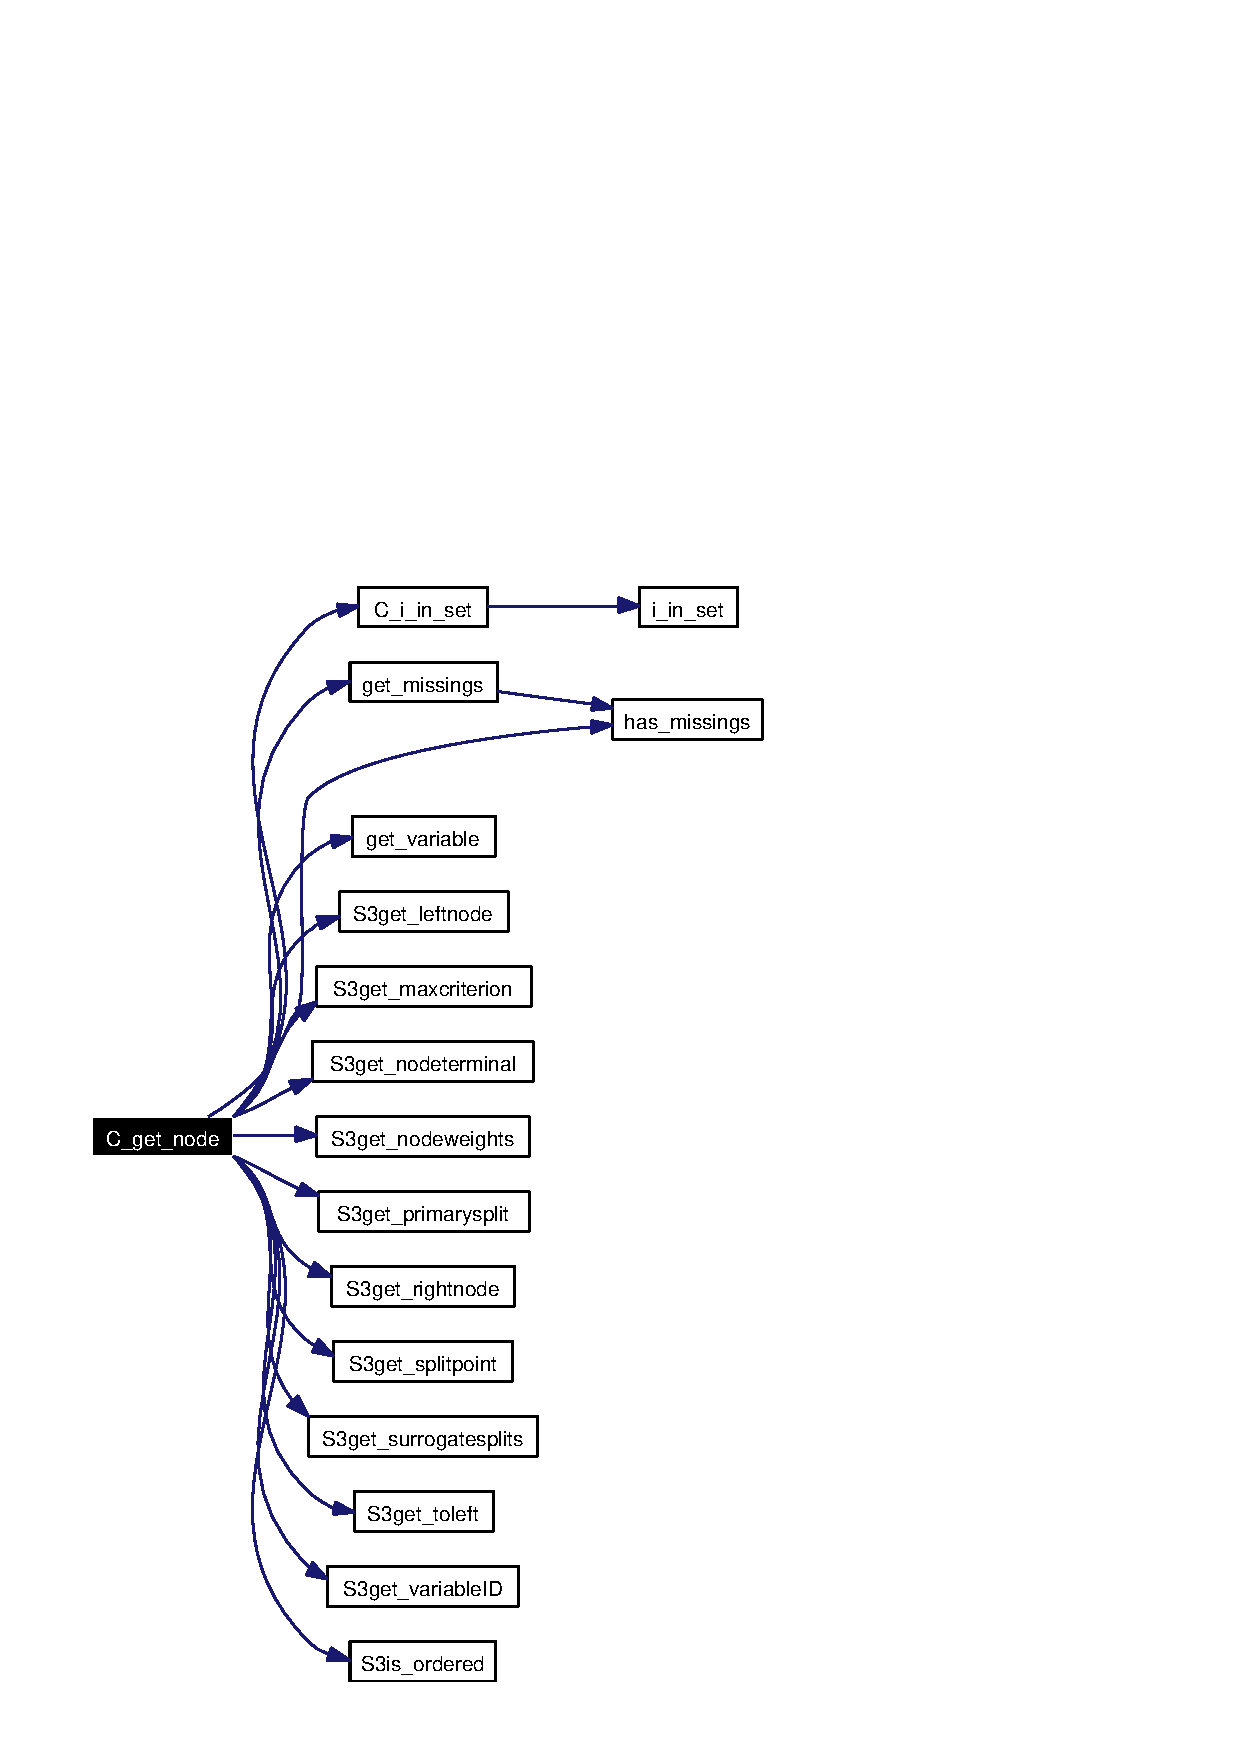
\includegraphics[width=187pt]{Predict_8c_a1_cgraph}
\end{center}
\end{figure}
\hypertarget{Predict_8c_a3}{
\index{Predict.c@{Predict.c}!C_get_nodebynum@{C\_\-get\_\-nodebynum}}
\index{C_get_nodebynum@{C\_\-get\_\-nodebynum}!Predict.c@{Predict.c}}
\subsubsection[C\_\-get\_\-nodebynum]{\setlength{\rightskip}{0pt plus 5cm}SEXP C\_\-get\_\-nodebynum (SEXP {\em subtree}, int {\em nodenum})}}
\label{Predict_8c_a3}


Get the node with node\-ID `nodenum' \par
 \begin{Desc}
\item[Parameters:]
\begin{description}
\item[{\em subtree}]a tree \item[{\em nodenum}]a node\-ID \end{description}
\end{Desc}


Definition at line 252 of file Predict.c.

References S3get\_\-leftnode(), S3get\_\-node\-ID(), S3get\_\-nodeterminal(), and S3get\_\-rightnode().

Referenced by C\_\-getpredictions(), C\_\-getweights(), R\_\-get\_\-nodebynum(), R\_\-predict\-RF(), R\_\-predict\-RF2(), and R\_\-predict\-RF\_\-weights().

Here is the call graph for this function:\begin{figure}[H]
\begin{center}
\leavevmode
\includegraphics[width=150pt]{Predict_8c_a3_cgraph}
\end{center}
\end{figure}
\hypertarget{Predict_8c_a7}{
\index{Predict.c@{Predict.c}!C_get_nodeID@{C\_\-get\_\-nodeID}}
\index{C_get_nodeID@{C\_\-get\_\-nodeID}!Predict.c@{Predict.c}}
\subsubsection[C\_\-get\_\-nodeID]{\setlength{\rightskip}{0pt plus 5cm}int C\_\-get\_\-node\-ID (SEXP {\em subtree}, SEXP {\em newinputs}, double {\em mincriterion}, int {\em numobs})}}
\label{Predict_8c_a7}


Get the node\-ID for a new observation \par
 \begin{Desc}
\item[Parameters:]
\begin{description}
\item[{\em subtree}]a tree \item[{\em newinputs}]an object of class `Variable\-Frame' \item[{\em mincriterion}]overwrites mincriterion used for tree growing \item[{\em numobs}]observation number \end{description}
\end{Desc}


Definition at line 316 of file Predict.c.

References C\_\-get\_\-node(), and S3get\_\-node\-ID().

Referenced by R\_\-get\_\-node\-ID(), R\_\-predict\-RF(), R\_\-predict\-RF2(), and R\_\-predict\-RF\_\-weights().

Here is the call graph for this function:\begin{figure}[H]
\begin{center}
\leavevmode
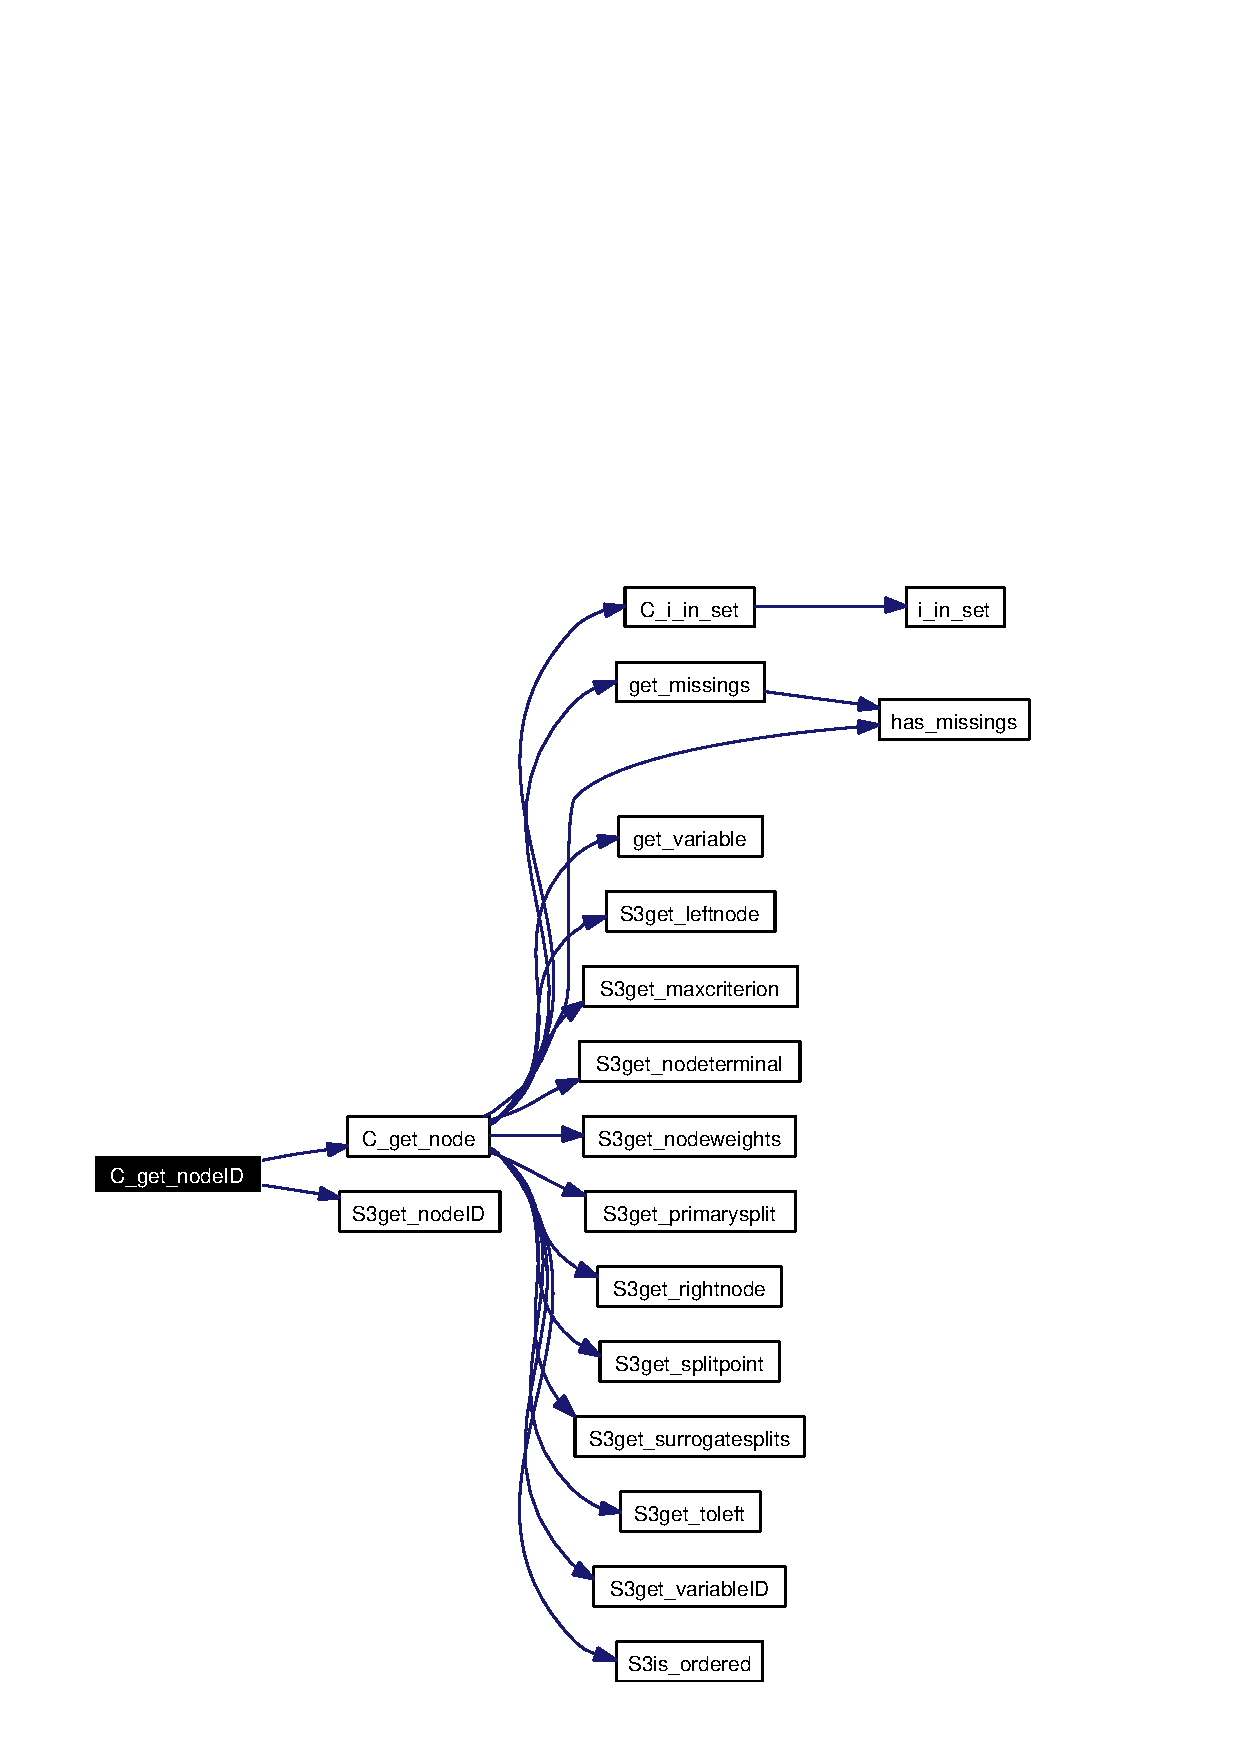
\includegraphics[width=251pt]{Predict_8c_a7_cgraph}
\end{center}
\end{figure}
\hypertarget{Predict_8c_a6}{
\index{Predict.c@{Predict.c}!C_get_nodeweights@{C\_\-get\_\-nodeweights}}
\index{C_get_nodeweights@{C\_\-get\_\-nodeweights}!Predict.c@{Predict.c}}
\subsubsection[C\_\-get\_\-nodeweights]{\setlength{\rightskip}{0pt plus 5cm}SEXP C\_\-get\_\-nodeweights (SEXP {\em subtree}, SEXP {\em newinputs}, double {\em mincriterion}, int {\em numobs})}}
\label{Predict_8c_a6}


Get the weights for a new observation \par
 \begin{Desc}
\item[Parameters:]
\begin{description}
\item[{\em subtree}]a tree \item[{\em newinputs}]an object of class `Variable\-Frame' \item[{\em mincriterion}]overwrites mincriterion used for tree growing \item[{\em numobs}]observation number \end{description}
\end{Desc}


Definition at line 301 of file Predict.c.

References C\_\-get\_\-node(), and S3get\_\-nodeweights().

Referenced by C\_\-weights().

Here is the call graph for this function:\begin{figure}[H]
\begin{center}
\leavevmode
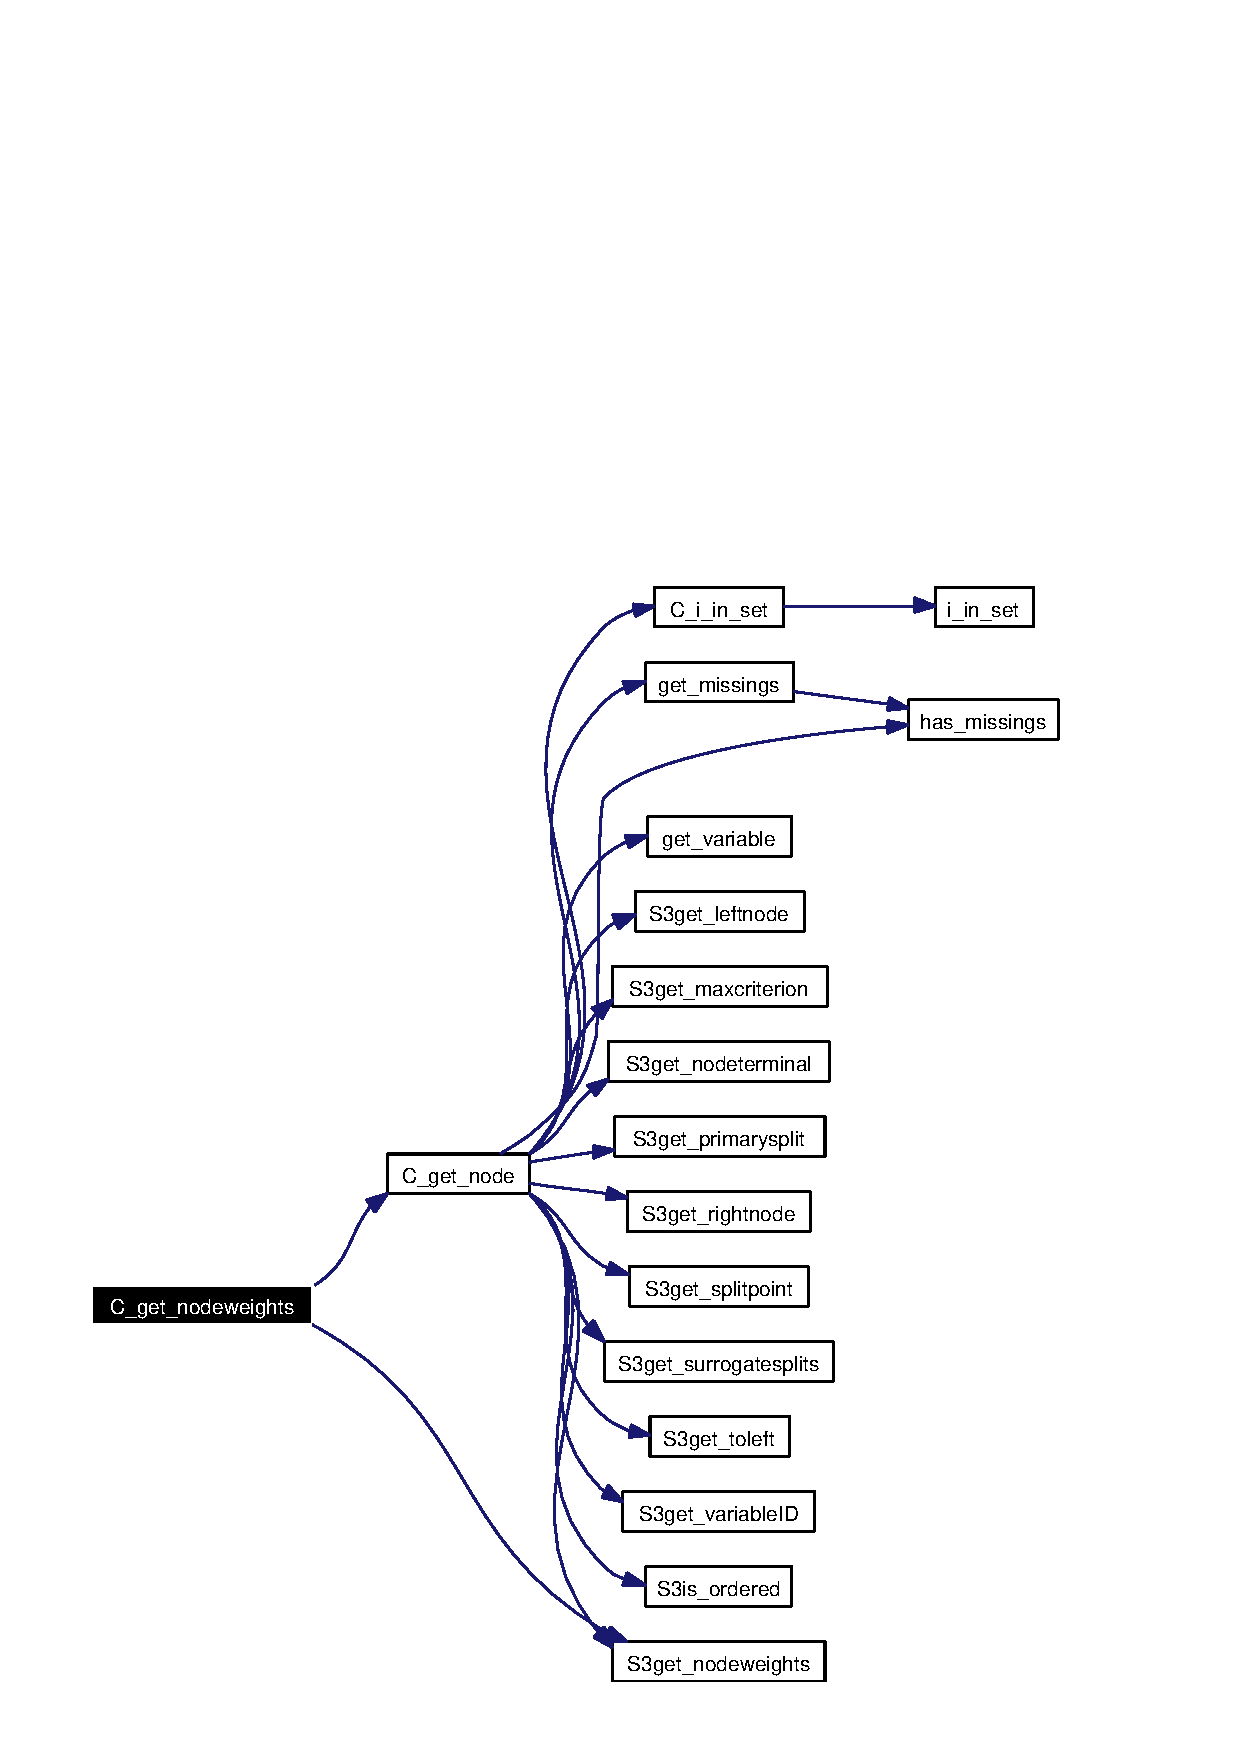
\includegraphics[width=258pt]{Predict_8c_a6_cgraph}
\end{center}
\end{figure}
\hypertarget{Predict_8c_a5}{
\index{Predict.c@{Predict.c}!C_get_prediction@{C\_\-get\_\-prediction}}
\index{C_get_prediction@{C\_\-get\_\-prediction}!Predict.c@{Predict.c}}
\subsubsection[C\_\-get\_\-prediction]{\setlength{\rightskip}{0pt plus 5cm}SEXP C\_\-get\_\-prediction (SEXP {\em subtree}, SEXP {\em newinputs}, double {\em mincriterion}, int {\em numobs})}}
\label{Predict_8c_a5}


Get the prediction of a new observation\par
 \begin{Desc}
\item[Parameters:]
\begin{description}
\item[{\em subtree}]a tree \item[{\em newinputs}]an object of class `Variable\-Frame' \item[{\em mincriterion}]overwrites mincriterion used for tree growing \item[{\em numobs}]observation number \end{description}
\end{Desc}


Definition at line 286 of file Predict.c.

References C\_\-get\_\-node(), and S3get\_\-prediction().

Referenced by C\_\-predict().

Here is the call graph for this function:\begin{figure}[H]
\begin{center}
\leavevmode
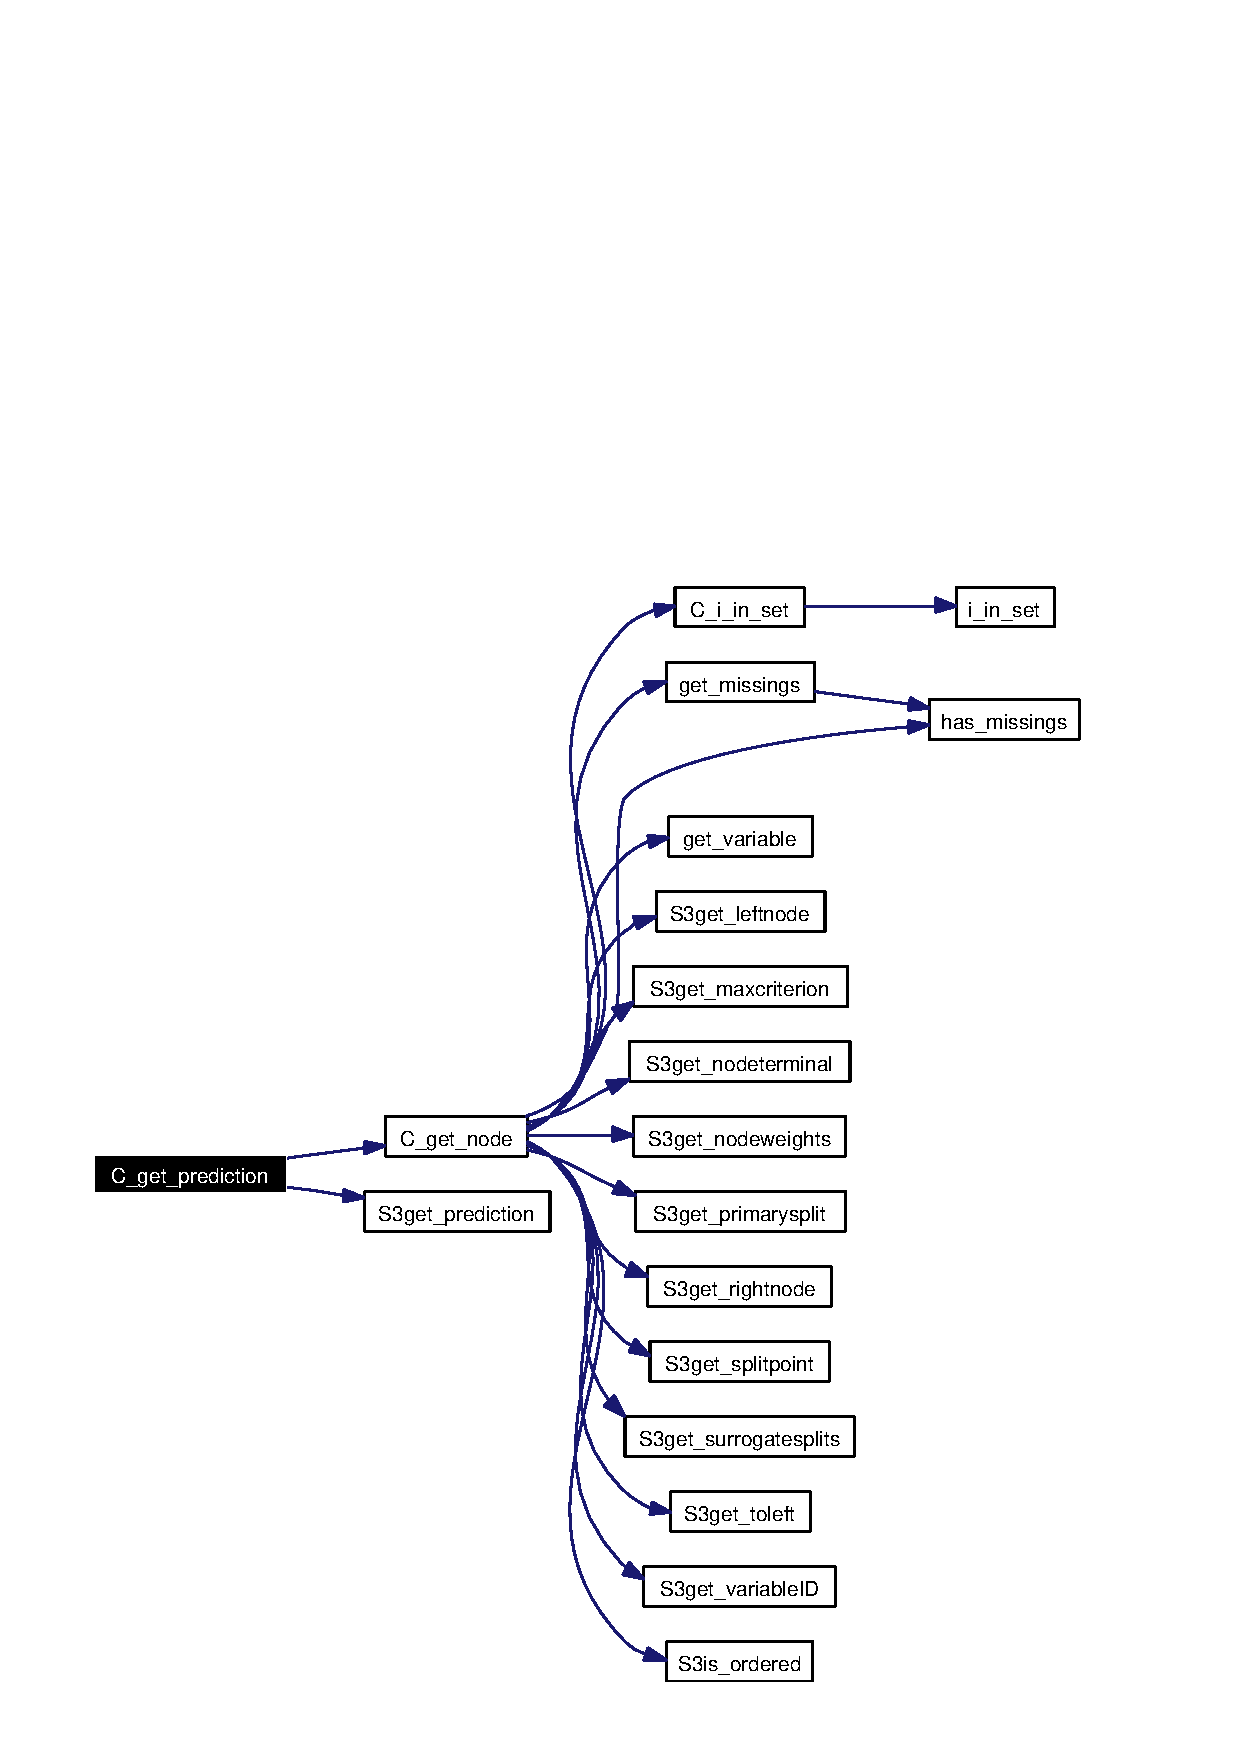
\includegraphics[width=263pt]{Predict_8c_a5_cgraph}
\end{center}
\end{figure}
\hypertarget{Predict_8c_a11}{
\index{Predict.c@{Predict.c}!C_getpredictions@{C\_\-getpredictions}}
\index{C_getpredictions@{C\_\-getpredictions}!Predict.c@{Predict.c}}
\subsubsection[C\_\-getpredictions]{\setlength{\rightskip}{0pt plus 5cm}void C\_\-getpredictions (SEXP {\em tree}, SEXP {\em where}, SEXP {\em ans})}}
\label{Predict_8c_a11}


Get the predictions from `where' nodes\par
 \begin{Desc}
\item[Parameters:]
\begin{description}
\item[{\em tree}]a tree \item[{\em where}]vector of node\-ID's \item[{\em ans}]return value \end{description}
\end{Desc}


Definition at line 394 of file Predict.c.

References C\_\-get\_\-nodebynum(), and S3get\_\-prediction().

Referenced by R\_\-getpredictions().

Here is the call graph for this function:\begin{figure}[H]
\begin{center}
\leavevmode
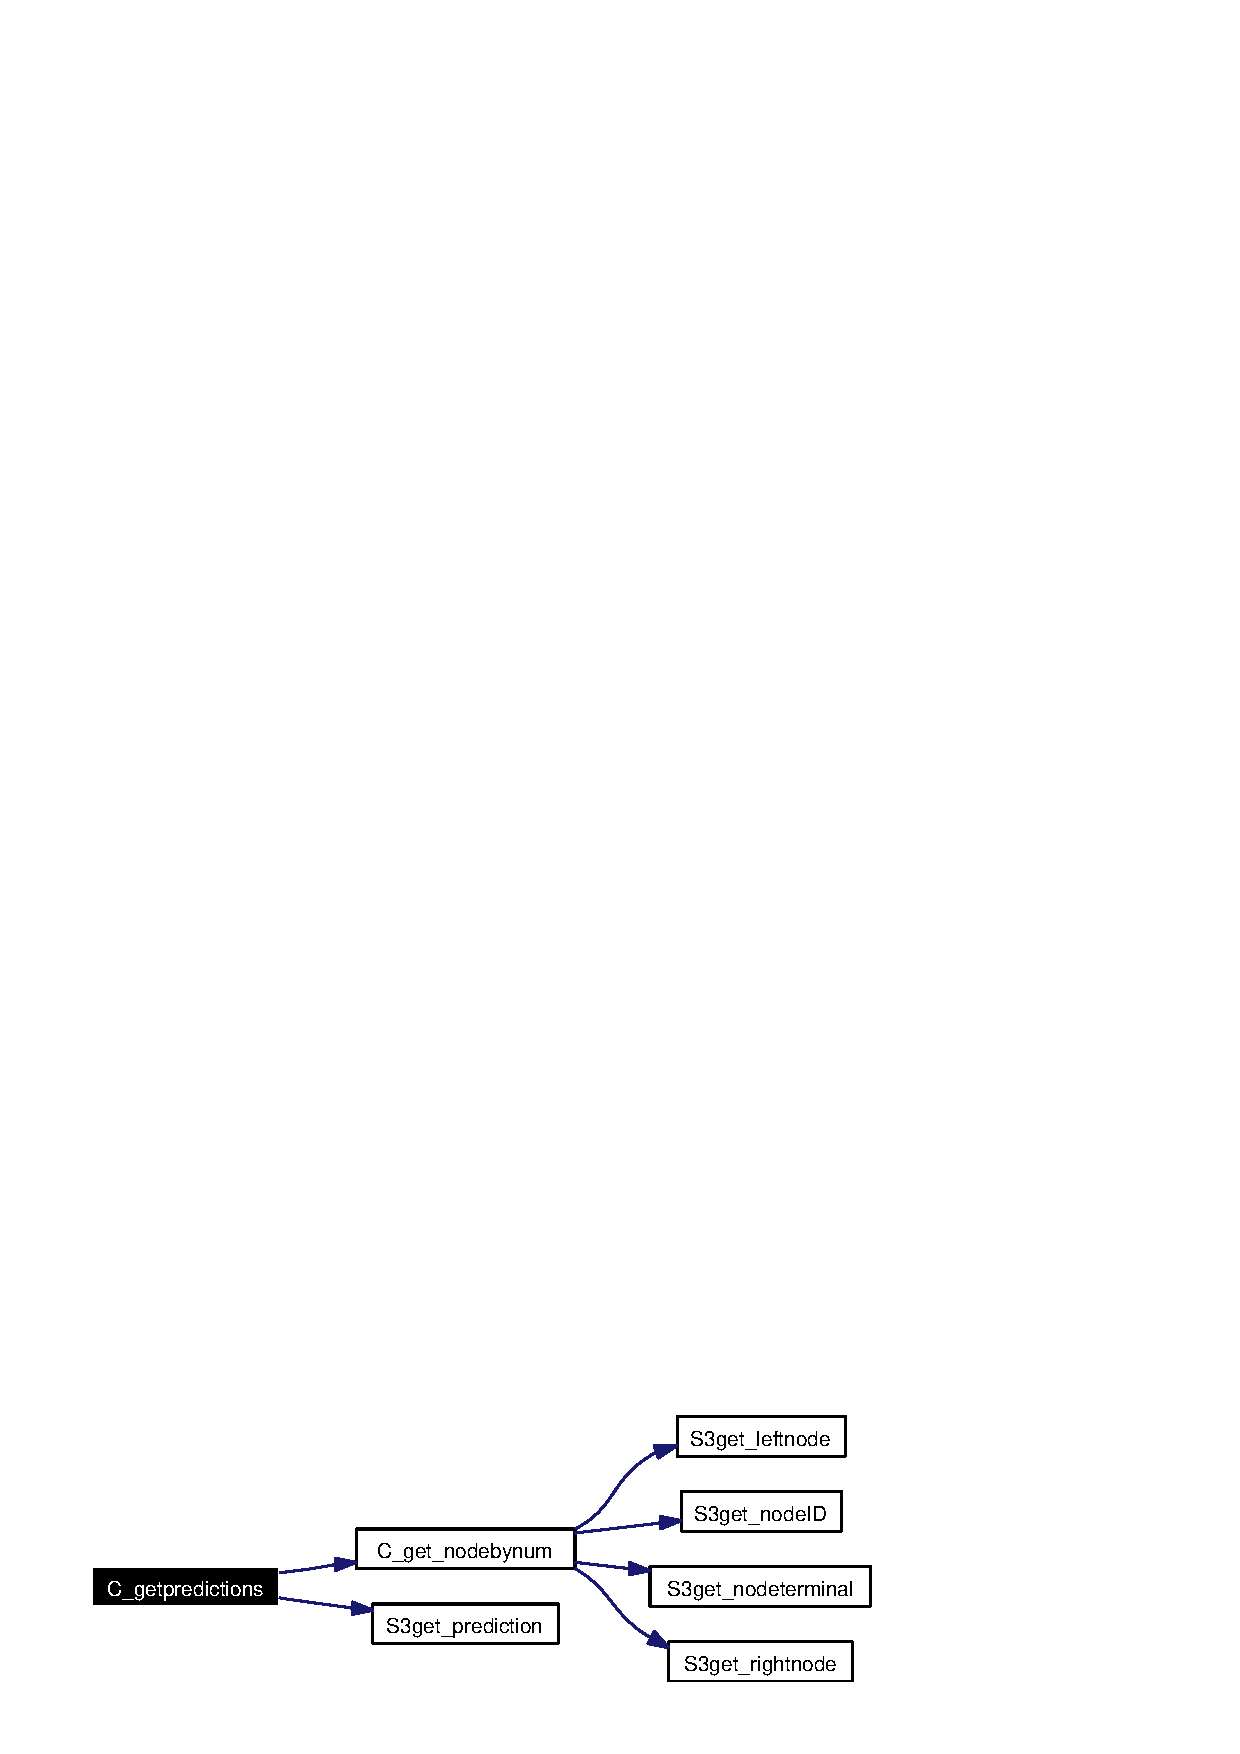
\includegraphics[width=213pt]{Predict_8c_a11_cgraph}
\end{center}
\end{figure}
\hypertarget{Predict_8c_a13}{
\index{Predict.c@{Predict.c}!C_getweights@{C\_\-getweights}}
\index{C_getweights@{C\_\-getweights}!Predict.c@{Predict.c}}
\subsubsection[C\_\-getweights]{\setlength{\rightskip}{0pt plus 5cm}void C\_\-getweights (SEXP {\em tree}, SEXP {\em where}, SEXP {\em ans})}}
\label{Predict_8c_a13}


Get the weights from `where' nodes\par
 \begin{Desc}
\item[Parameters:]
\begin{description}
\item[{\em tree}]a tree \item[{\em where}]vector of node\-ID's \item[{\em ans}]return value \end{description}
\end{Desc}


Definition at line 435 of file Predict.c.

References C\_\-get\_\-nodebynum(), and S3get\_\-nodeweights().

Referenced by R\_\-getweights().

Here is the call graph for this function:\begin{figure}[H]
\begin{center}
\leavevmode
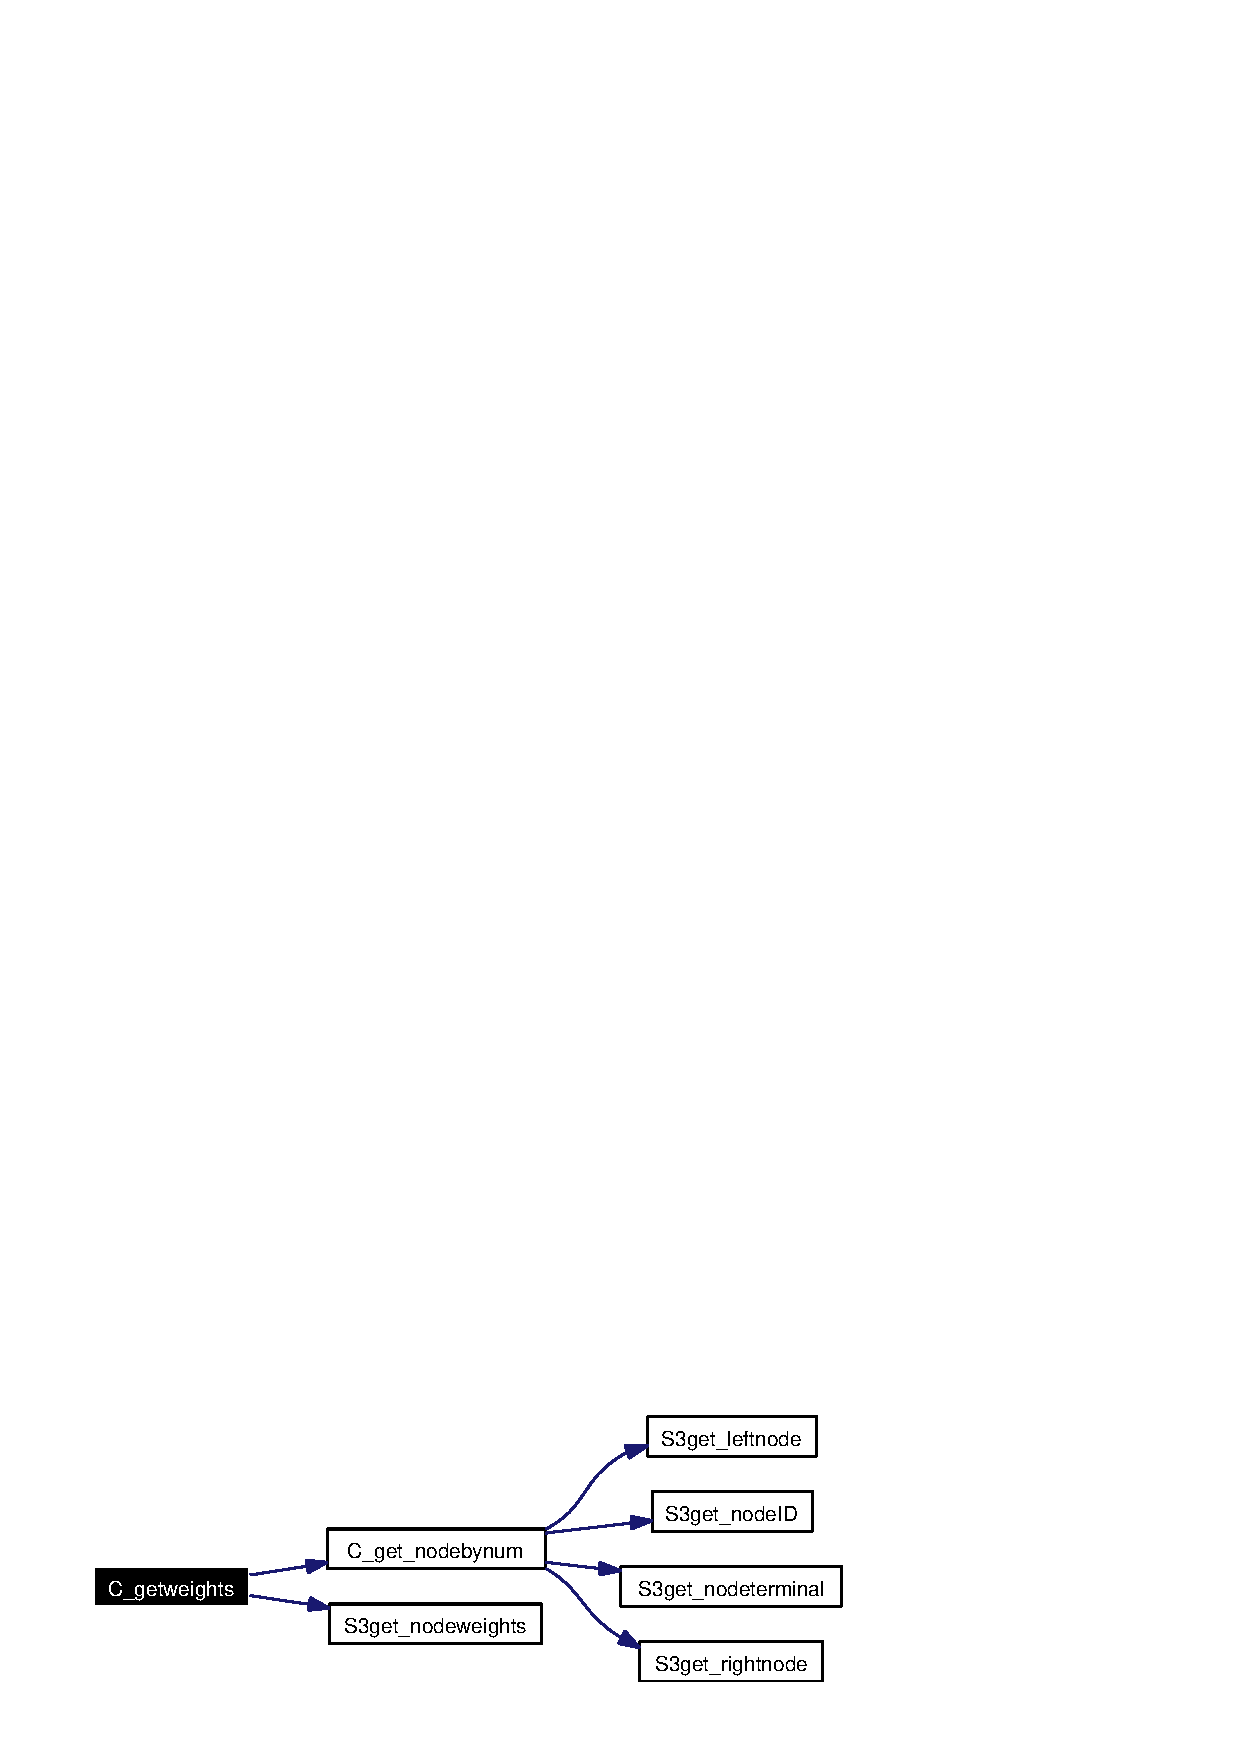
\includegraphics[width=206pt]{Predict_8c_a13_cgraph}
\end{center}
\end{figure}
\hypertarget{Predict_8c_a9}{
\index{Predict.c@{Predict.c}!C_predict@{C\_\-predict}}
\index{C_predict@{C\_\-predict}!Predict.c@{Predict.c}}
\subsubsection[C\_\-predict]{\setlength{\rightskip}{0pt plus 5cm}void C\_\-predict (SEXP {\em tree}, SEXP {\em newinputs}, double {\em mincriterion}, SEXP {\em ans})}}
\label{Predict_8c_a9}


Get all predictions for `newinputs' \par
 \begin{Desc}
\item[Parameters:]
\begin{description}
\item[{\em tree}]a tree \item[{\em newinputs}]an object of class `Variable\-Frame' \item[{\em mincriterion}]overwrites mincriterion used for tree growing \item[{\em ans}]return value \end{description}
\end{Desc}


Definition at line 353 of file Predict.c.

References C\_\-get\_\-prediction(), and get\_\-nobs().

Referenced by R\_\-predict().

Here is the call graph for this function:\begin{figure}[H]
\begin{center}
\leavevmode
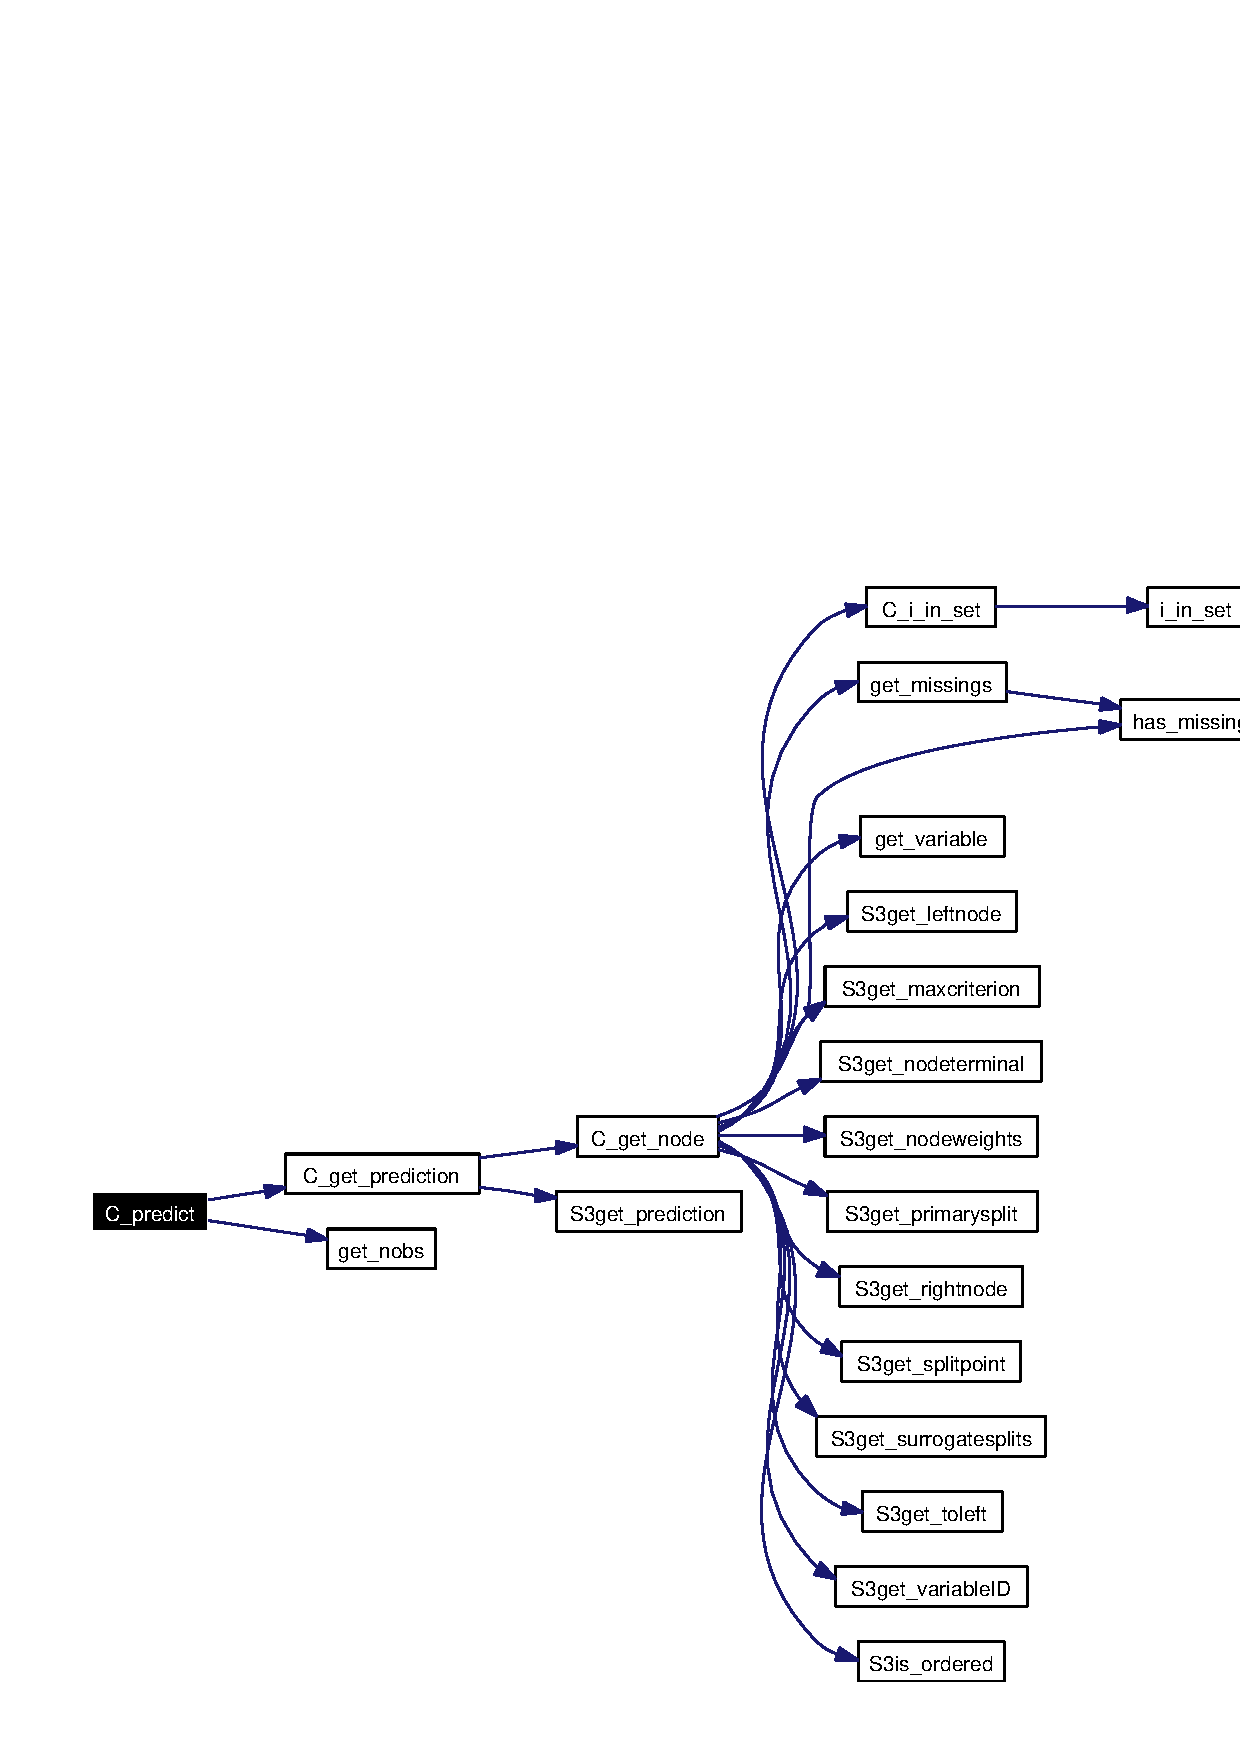
\includegraphics[width=309pt]{Predict_8c_a9_cgraph}
\end{center}
\end{figure}
\hypertarget{Predict_8c_a0}{
\index{Predict.c@{Predict.c}!C_splitnode@{C\_\-splitnode}}
\index{C_splitnode@{C\_\-splitnode}!Predict.c@{Predict.c}}
\subsubsection[C\_\-splitnode]{\setlength{\rightskip}{0pt plus 5cm}void C\_\-splitnode (SEXP {\em node}, SEXP {\em learnsample}, SEXP {\em control})}}
\label{Predict_8c_a0}


Split a node according to a splitting rule \par
 \begin{Desc}
\item[Parameters:]
\begin{description}
\item[{\em node}]the current node with primary split specified \item[{\em learnsample}]learning sample \item[{\em control}]an object of class `Tree\-Control' \end{description}
\end{Desc}
\begin{Desc}
\item[\hyperlink{todo__todo000001}{Todo}]outplace the splitting since there are at least 3 functions with nearly identical code \end{Desc}


Definition at line 21 of file Predict.c.

References C\_\-init\_\-node(), get\_\-maxsurrogate(), get\_\-missings(), get\_\-ninputs(), get\_\-nobs(), get\_\-splitctrl(), get\_\-variable(), has\_\-missings(), i\_\-in\_\-set(), ncol(), NODE\_\-LENGTH, PL2\_\-inputs\-Sym, PL2\_\-jointtransf\-Sym, PL2\_\-responses\-Sym, S3\_\-LEFT, S3\_\-RIGHT, S3get\_\-nodeweights(), S3get\_\-primarysplit(), S3get\_\-splitpoint(), S3get\_\-variable\-ID(), and S3is\_\-ordered().

Referenced by C\_\-Tree\-Grow().

Here is the call graph for this function:\begin{figure}[H]
\begin{center}
\leavevmode
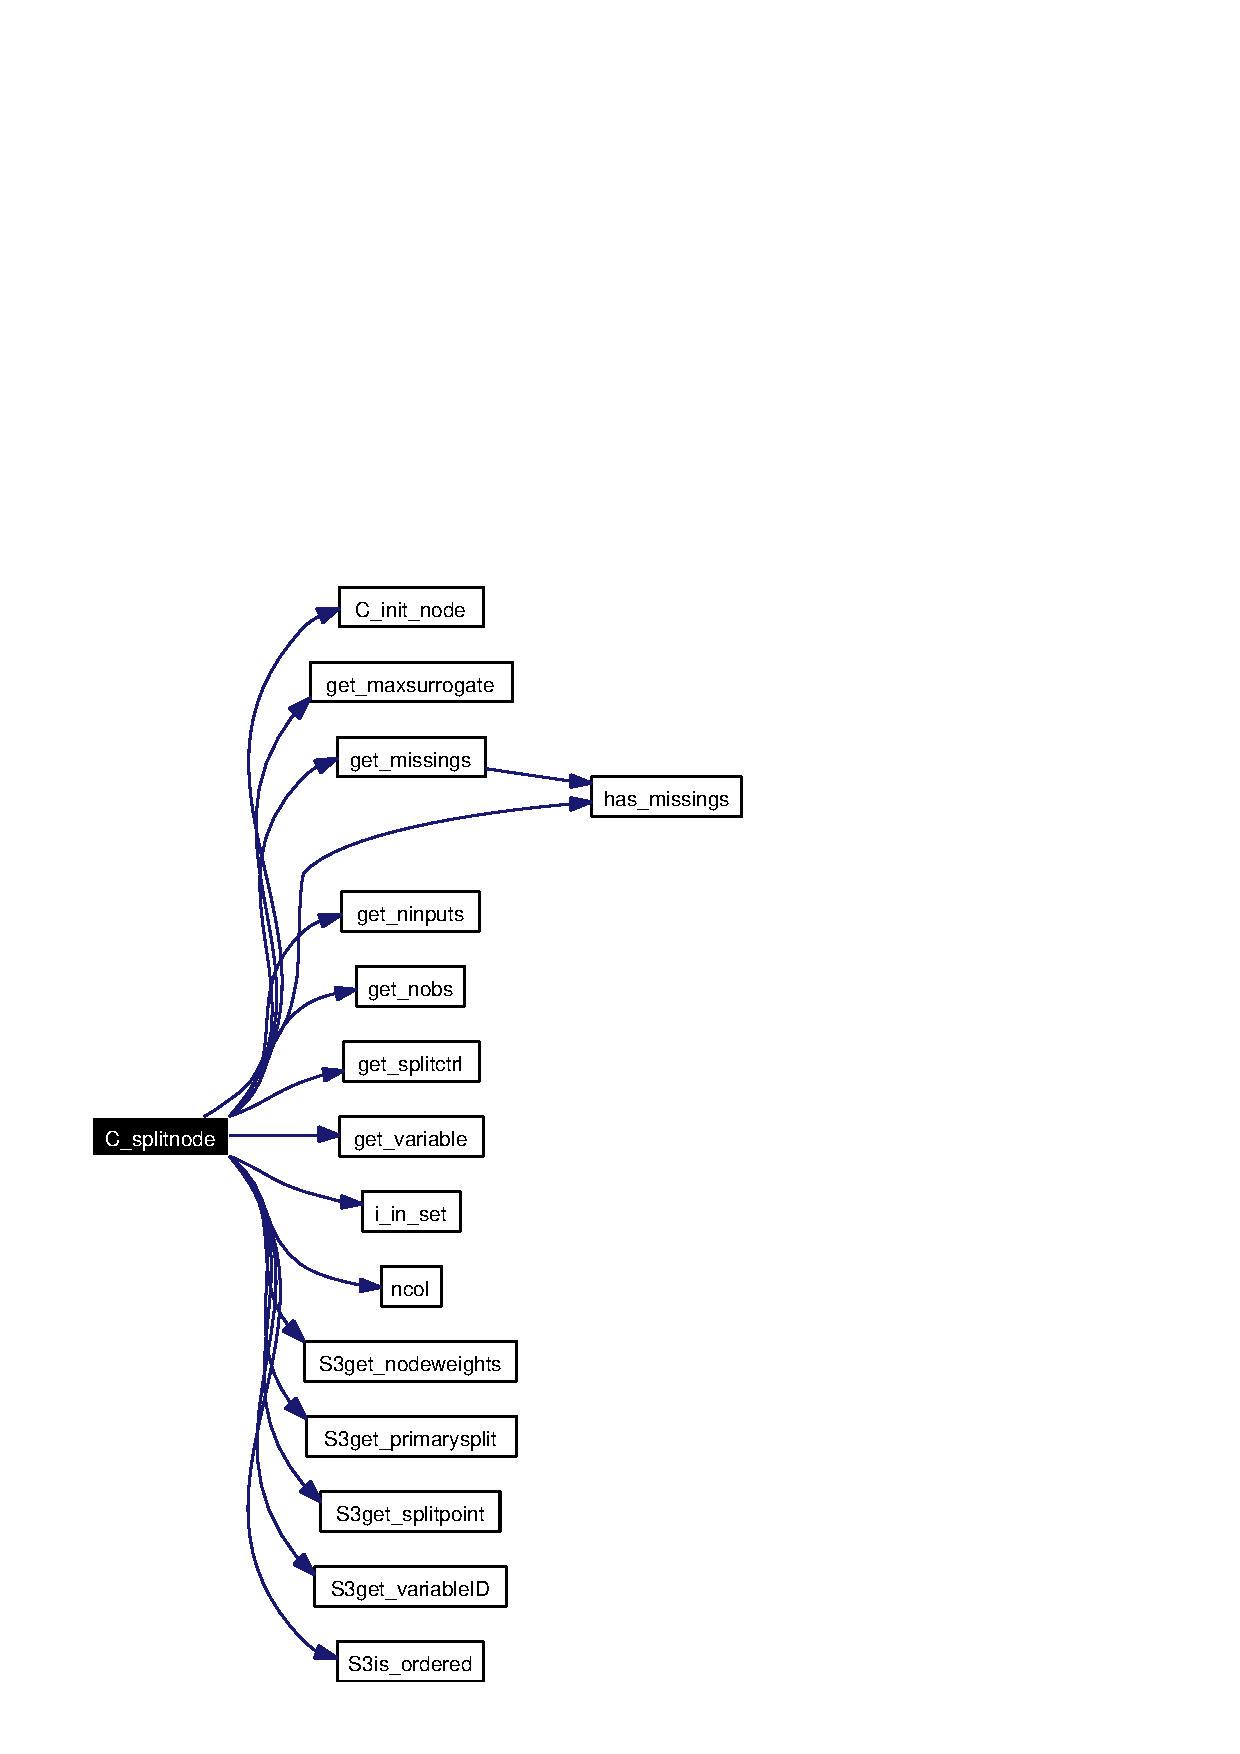
\includegraphics[width=182pt]{Predict_8c_a0_cgraph}
\end{center}
\end{figure}
\hypertarget{Predict_8c_a15}{
\index{Predict.c@{Predict.c}!C_weights@{C\_\-weights}}
\index{C_weights@{C\_\-weights}!Predict.c@{Predict.c}}
\subsubsection[C\_\-weights]{\setlength{\rightskip}{0pt plus 5cm}void C\_\-weights (SEXP {\em tree}, SEXP {\em newinputs}, double {\em mincriterion}, SEXP {\em ans})}}
\label{Predict_8c_a15}


Get the weights for all observations in `newinputs' \begin{Desc}
\item[Parameters:]
\begin{description}
\item[{\em tree}]a tree \item[{\em newinputs}]an object of class `Variable\-Frame' \item[{\em mincriterion}]overwrites mincriterion used for tree growing \item[{\em ans}]return value \end{description}
\end{Desc}


Definition at line 477 of file Predict.c.

References C\_\-get\_\-nodeweights(), and get\_\-nobs().

Referenced by R\_\-weights().

Here is the call graph for this function:\begin{figure}[H]
\begin{center}
\leavevmode
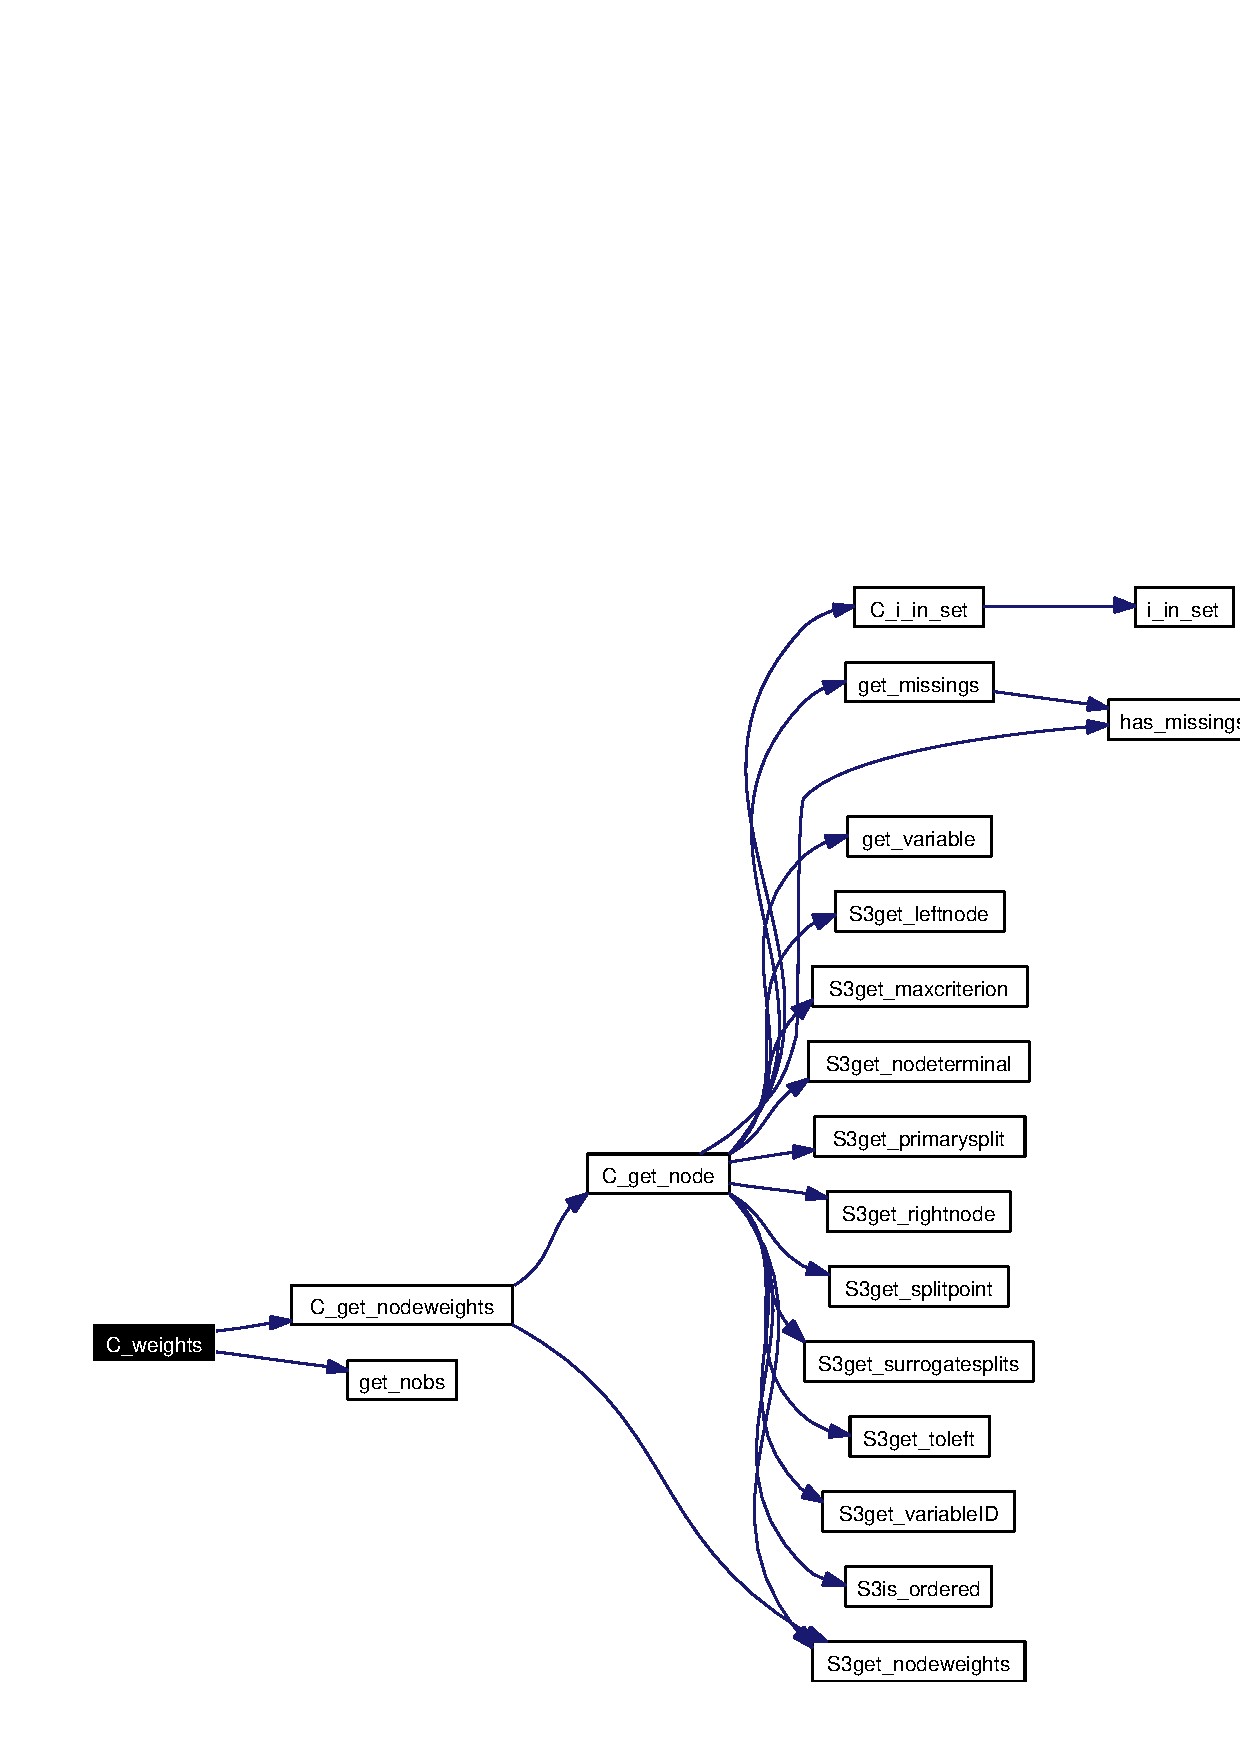
\includegraphics[width=306pt]{Predict_8c_a15_cgraph}
\end{center}
\end{figure}
\hypertarget{Predict_8c_a2}{
\index{Predict.c@{Predict.c}!R_get_node@{R\_\-get\_\-node}}
\index{R_get_node@{R\_\-get\_\-node}!Predict.c@{Predict.c}}
\subsubsection[R\_\-get\_\-node]{\setlength{\rightskip}{0pt plus 5cm}SEXP R\_\-get\_\-node (SEXP {\em subtree}, SEXP {\em newinputs}, SEXP {\em mincriterion}, SEXP {\em numobs})}}
\label{Predict_8c_a2}


R-Interface to C\_\-get\_\-node \par
 \begin{Desc}
\item[Parameters:]
\begin{description}
\item[{\em subtree}]a tree \item[{\em newinputs}]an object of class `Variable\-Frame' \item[{\em mincriterion}]overwrites mincriterion used for tree growing \item[{\em numobs}]observation number \end{description}
\end{Desc}


Definition at line 239 of file Predict.c.

References C\_\-get\_\-node().

Here is the call graph for this function:\begin{figure}[H]
\begin{center}
\leavevmode
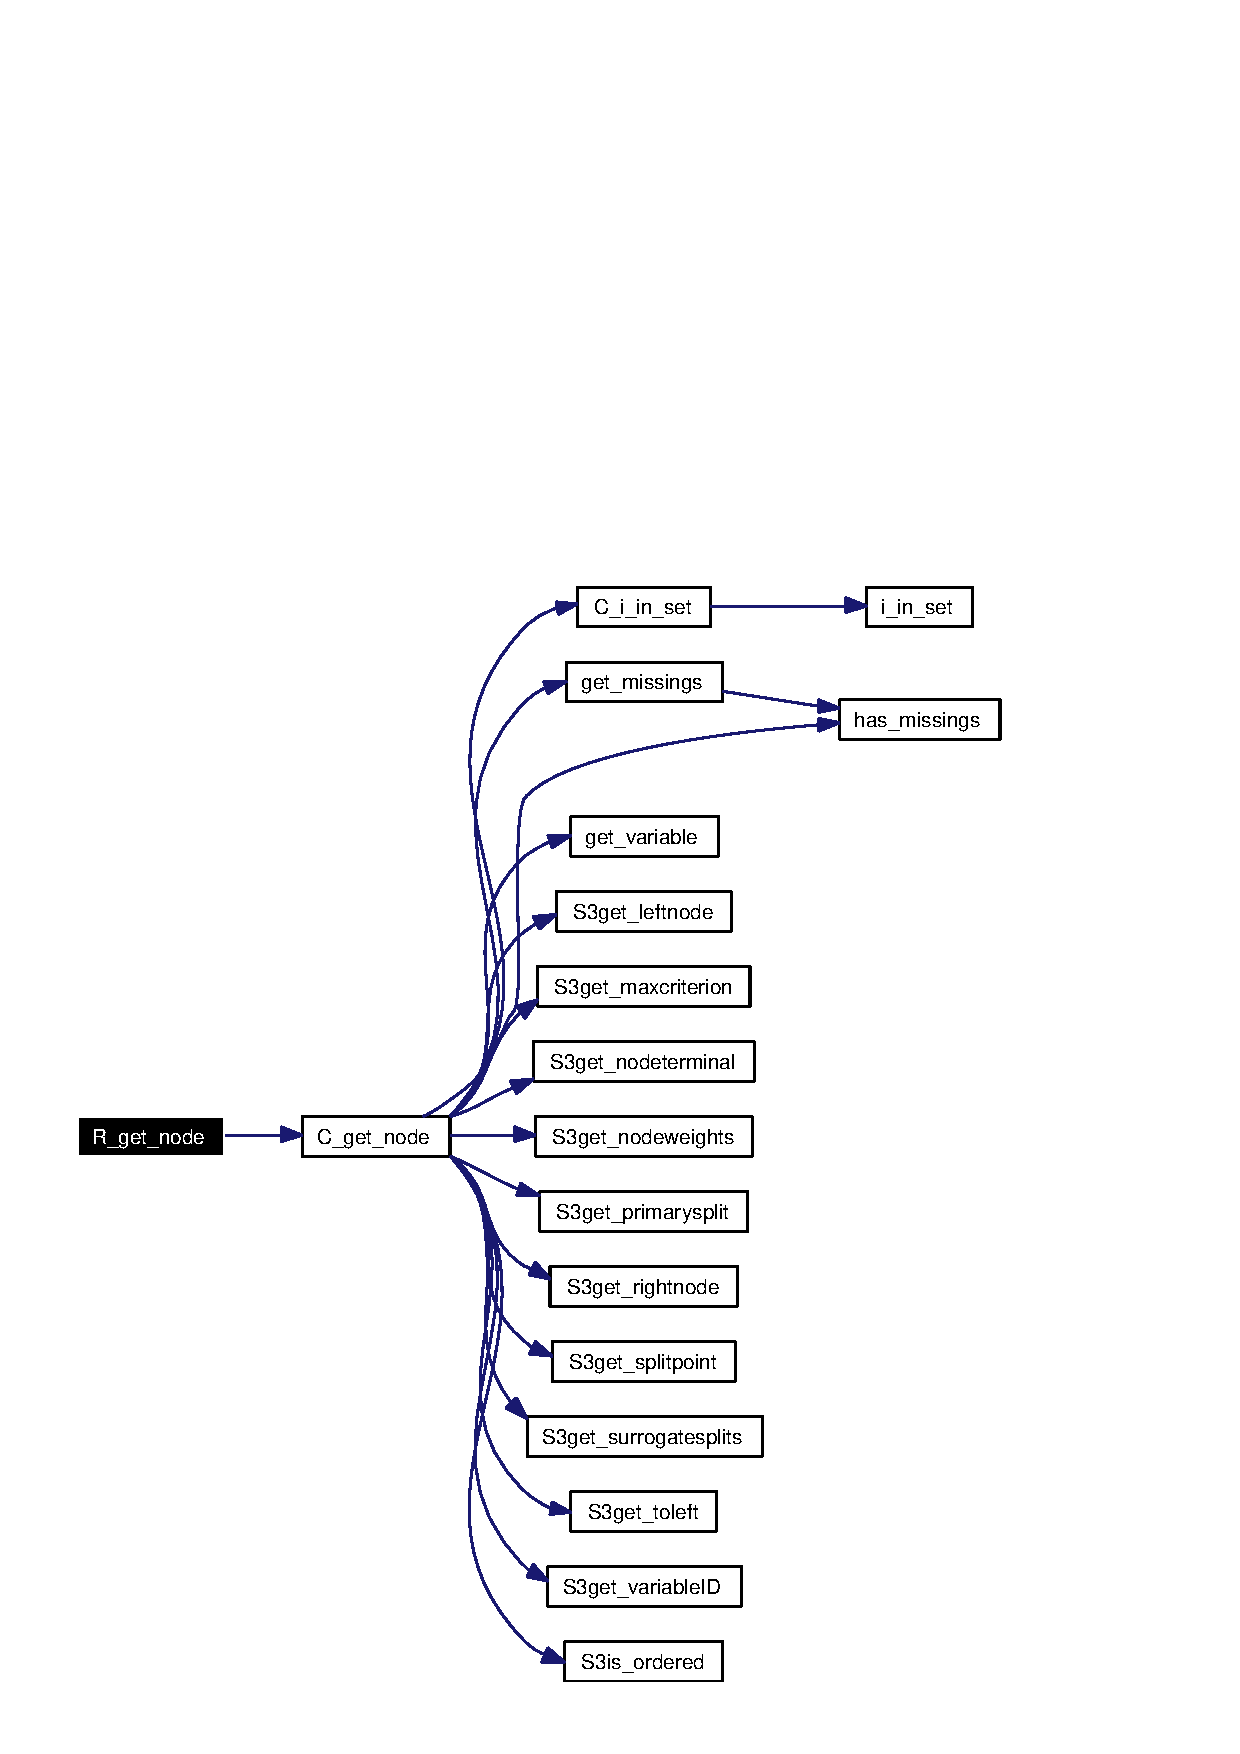
\includegraphics[width=240pt]{Predict_8c_a2_cgraph}
\end{center}
\end{figure}
\hypertarget{Predict_8c_a4}{
\index{Predict.c@{Predict.c}!R_get_nodebynum@{R\_\-get\_\-nodebynum}}
\index{R_get_nodebynum@{R\_\-get\_\-nodebynum}!Predict.c@{Predict.c}}
\subsubsection[R\_\-get\_\-nodebynum]{\setlength{\rightskip}{0pt plus 5cm}SEXP R\_\-get\_\-nodebynum (SEXP {\em subtree}, SEXP {\em nodenum})}}
\label{Predict_8c_a4}


R-Interface to C\_\-get\_\-nodenum \par
 \begin{Desc}
\item[Parameters:]
\begin{description}
\item[{\em subtree}]a tree \item[{\em nodenum}]a node\-ID \end{description}
\end{Desc}


Definition at line 273 of file Predict.c.

References C\_\-get\_\-nodebynum().

Here is the call graph for this function:\begin{figure}[H]
\begin{center}
\leavevmode
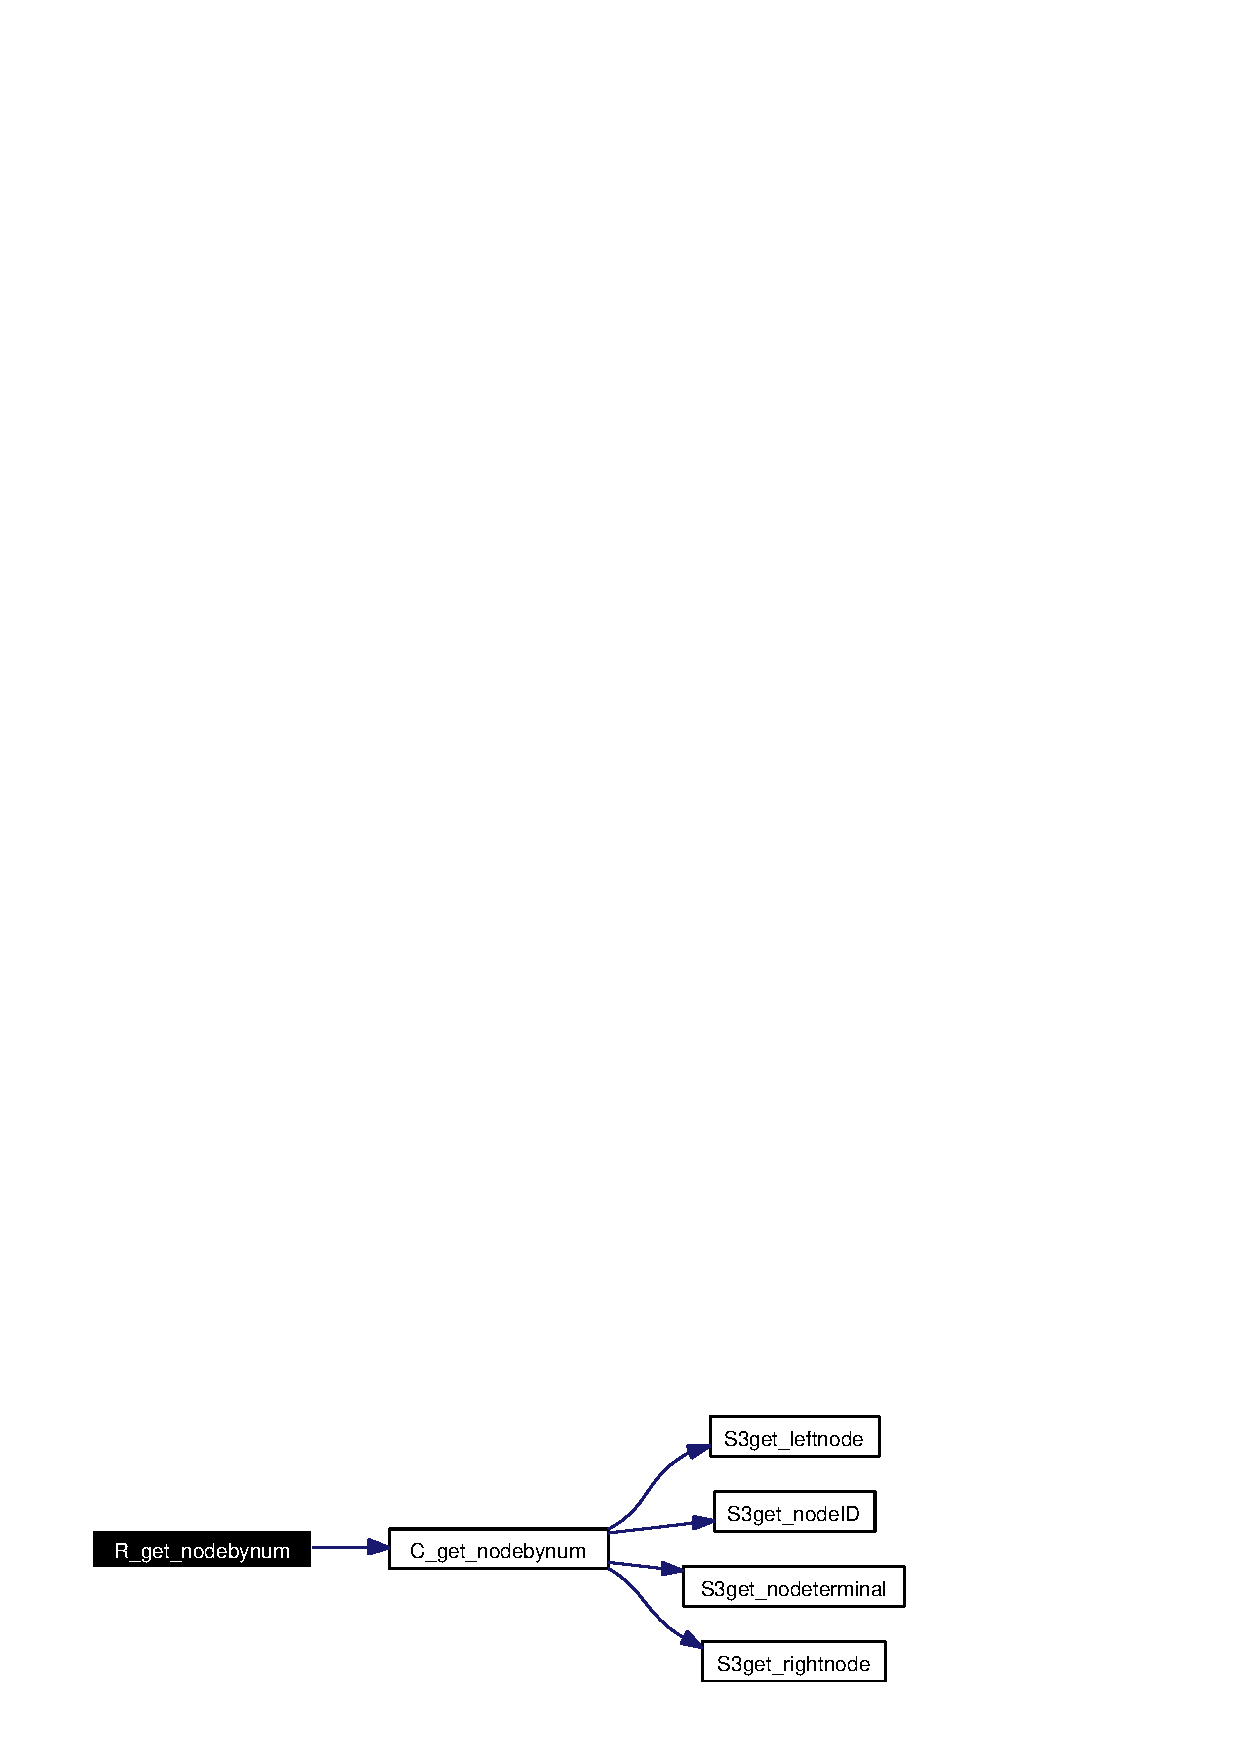
\includegraphics[width=221pt]{Predict_8c_a4_cgraph}
\end{center}
\end{figure}
\hypertarget{Predict_8c_a8}{
\index{Predict.c@{Predict.c}!R_get_nodeID@{R\_\-get\_\-nodeID}}
\index{R_get_nodeID@{R\_\-get\_\-nodeID}!Predict.c@{Predict.c}}
\subsubsection[R\_\-get\_\-nodeID]{\setlength{\rightskip}{0pt plus 5cm}SEXP R\_\-get\_\-node\-ID (SEXP {\em tree}, SEXP {\em newinputs}, SEXP {\em mincriterion})}}
\label{Predict_8c_a8}


R-Interface to C\_\-get\_\-node\-ID \par
 \begin{Desc}
\item[Parameters:]
\begin{description}
\item[{\em tree}]a tree \item[{\em newinputs}]an object of class `Variable\-Frame' \item[{\em mincriterion}]overwrites mincriterion used for tree growing \end{description}
\end{Desc}


Definition at line 330 of file Predict.c.

References C\_\-get\_\-node\-ID(), and get\_\-nobs().

Here is the call graph for this function:\begin{figure}[H]
\begin{center}
\leavevmode
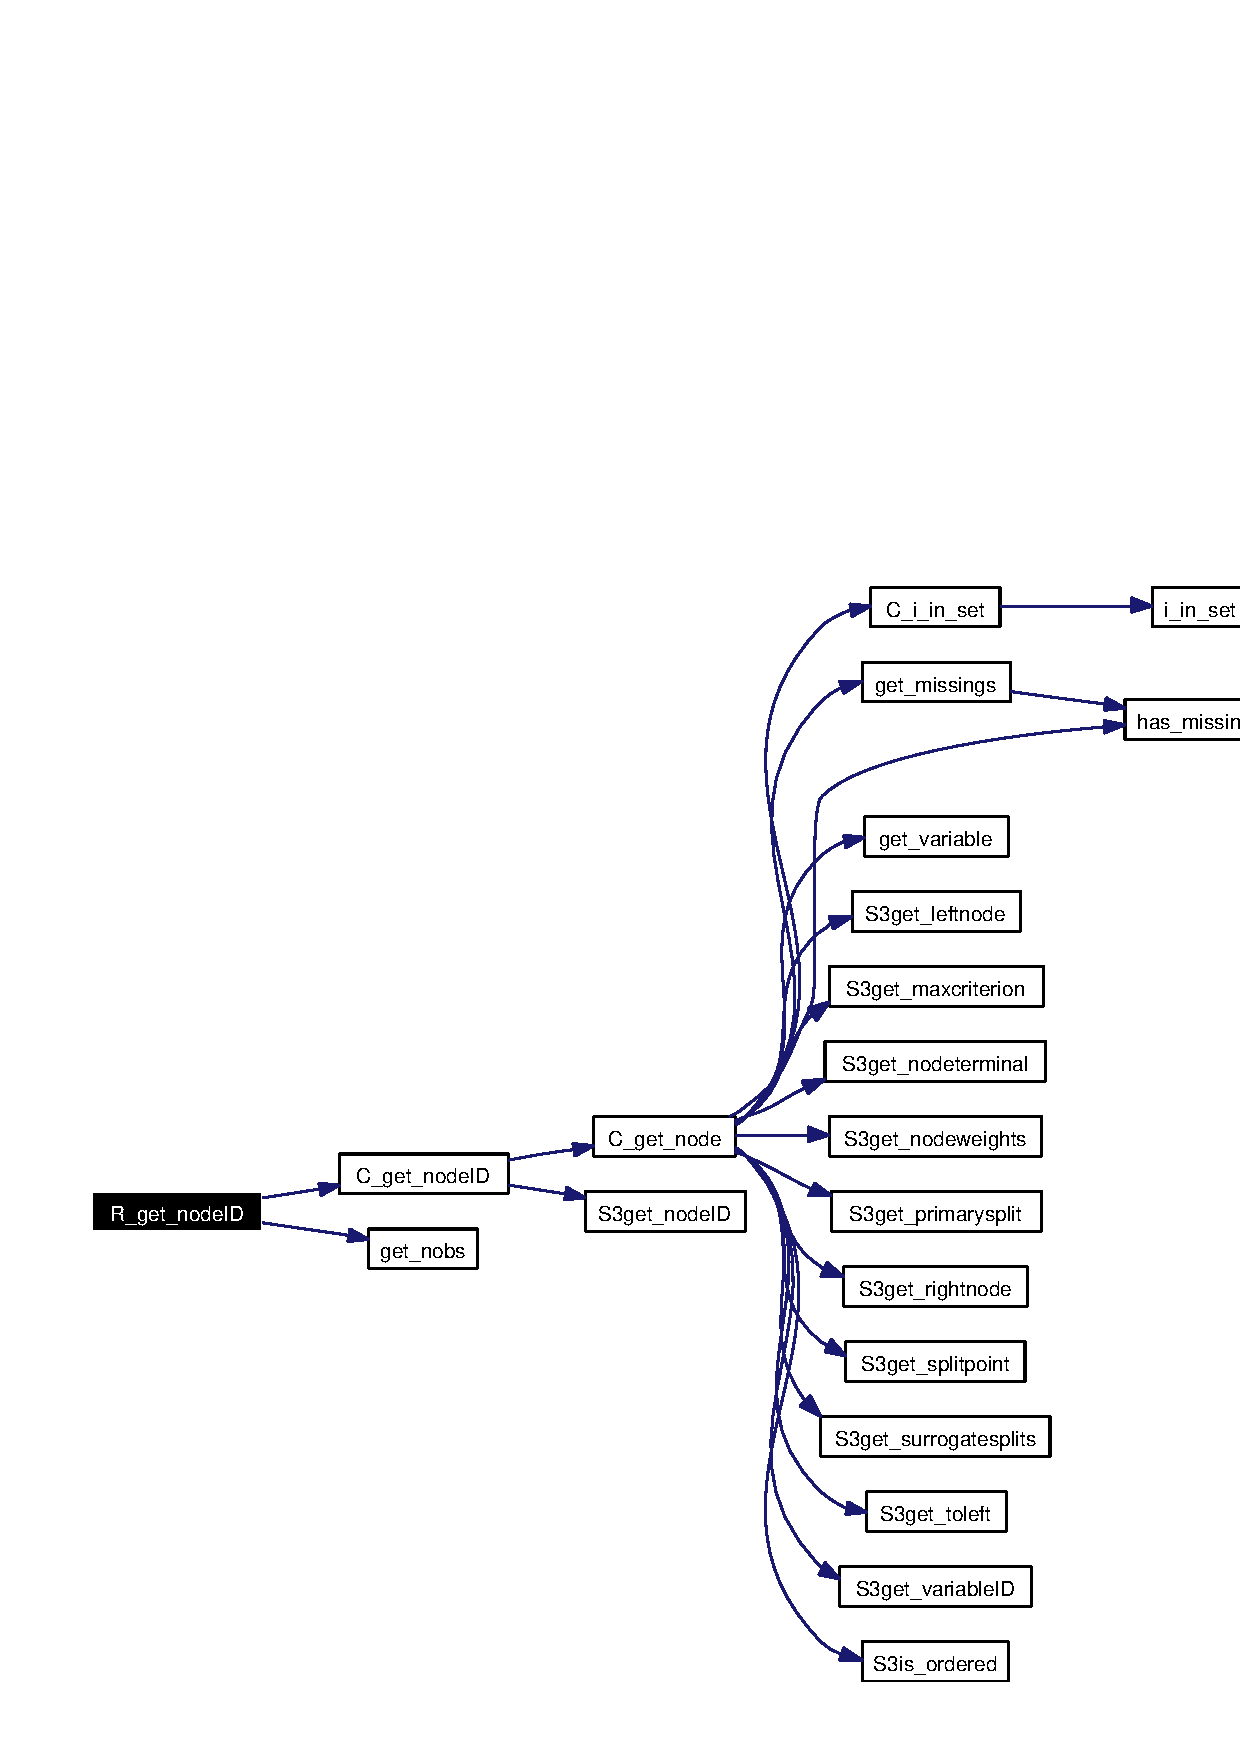
\includegraphics[width=310pt]{Predict_8c_a8_cgraph}
\end{center}
\end{figure}
\hypertarget{Predict_8c_a12}{
\index{Predict.c@{Predict.c}!R_getpredictions@{R\_\-getpredictions}}
\index{R_getpredictions@{R\_\-getpredictions}!Predict.c@{Predict.c}}
\subsubsection[R\_\-getpredictions]{\setlength{\rightskip}{0pt plus 5cm}SEXP R\_\-getpredictions (SEXP {\em tree}, SEXP {\em where})}}
\label{Predict_8c_a12}


R-Interface to C\_\-getpredictions\par
 \begin{Desc}
\item[Parameters:]
\begin{description}
\item[{\em tree}]a tree \item[{\em where}]vector of node\-ID's \end{description}
\end{Desc}


Definition at line 415 of file Predict.c.

References C\_\-getpredictions().

Here is the call graph for this function:\begin{figure}[H]
\begin{center}
\leavevmode
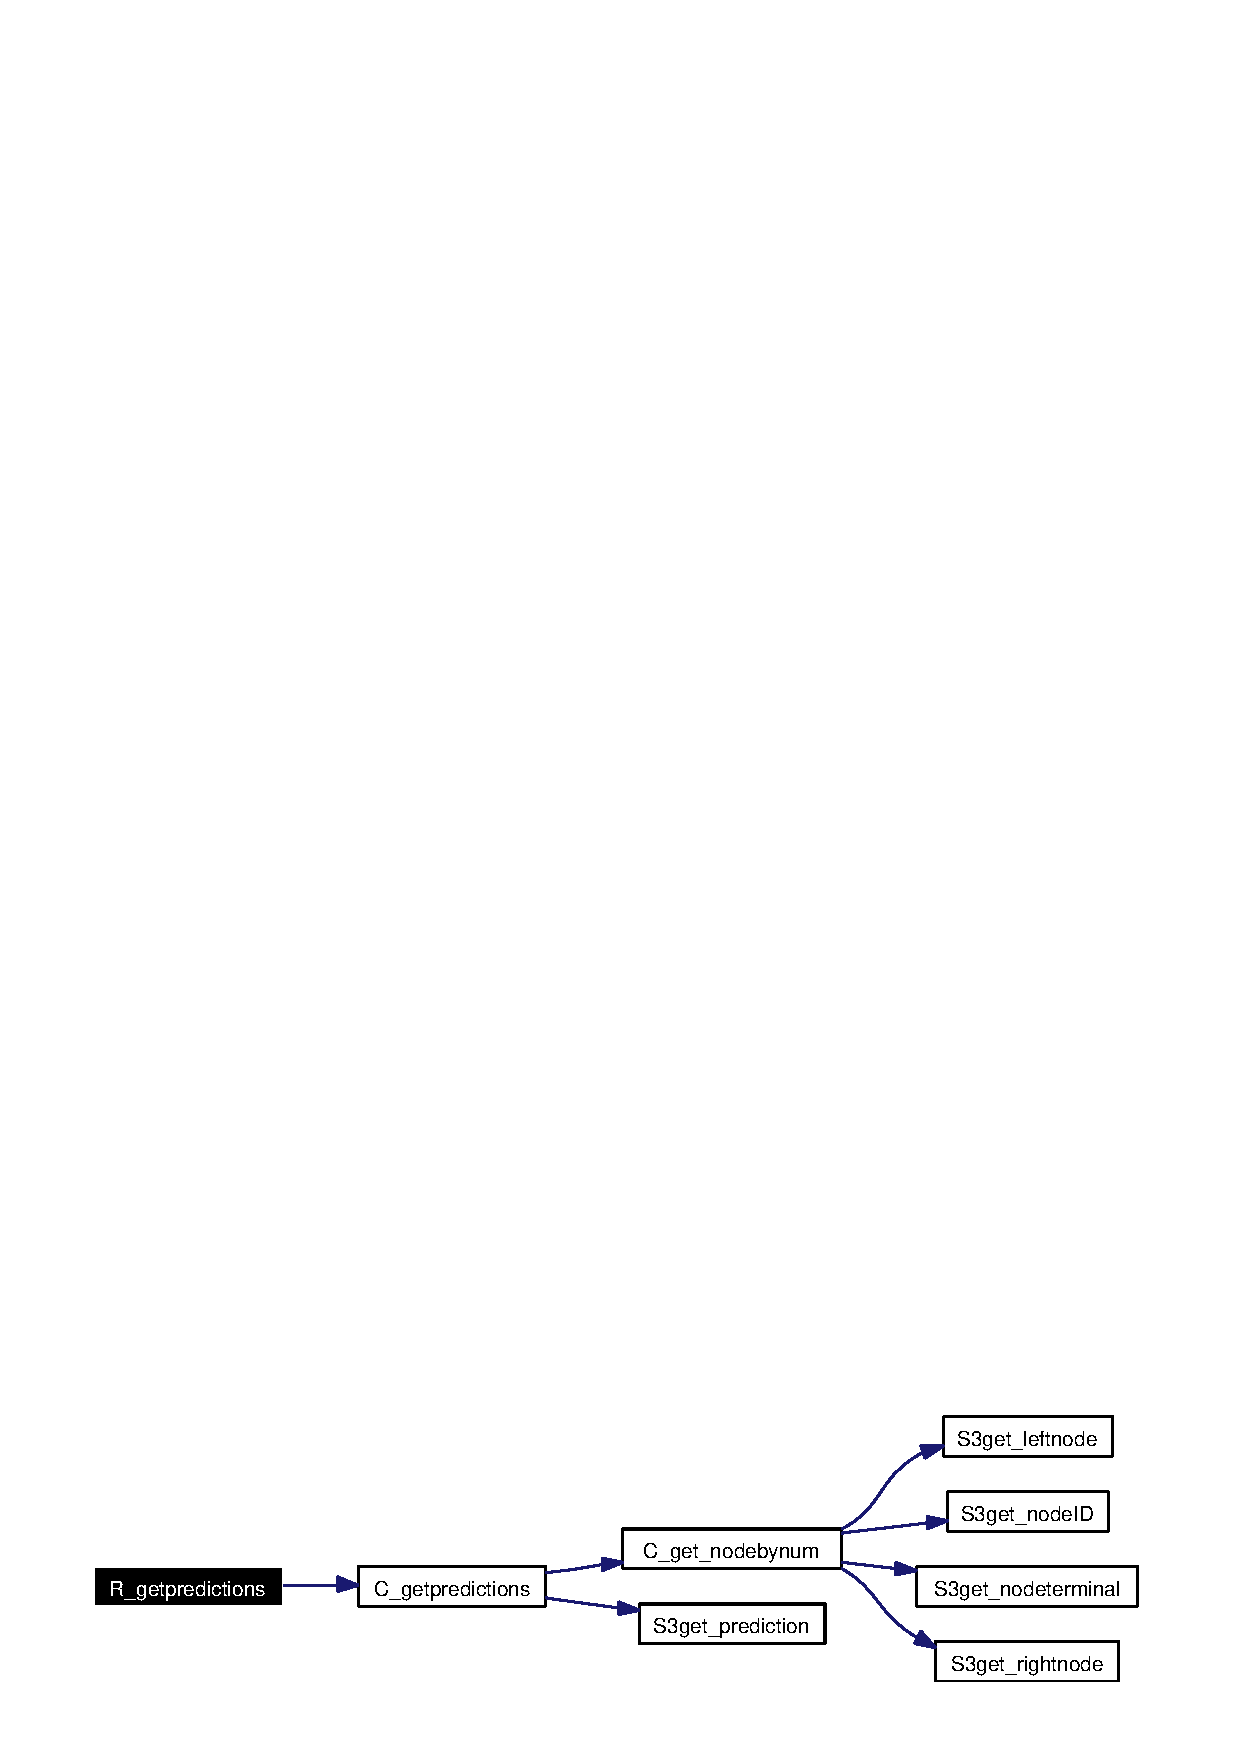
\includegraphics[width=277pt]{Predict_8c_a12_cgraph}
\end{center}
\end{figure}
\hypertarget{Predict_8c_a14}{
\index{Predict.c@{Predict.c}!R_getweights@{R\_\-getweights}}
\index{R_getweights@{R\_\-getweights}!Predict.c@{Predict.c}}
\subsubsection[R\_\-getweights]{\setlength{\rightskip}{0pt plus 5cm}SEXP R\_\-getweights (SEXP {\em tree}, SEXP {\em where})}}
\label{Predict_8c_a14}


R-Interface to C\_\-getweigts \par
 \begin{Desc}
\item[Parameters:]
\begin{description}
\item[{\em tree}]a tree \item[{\em where}]vector of node\-ID's \end{description}
\end{Desc}


Definition at line 456 of file Predict.c.

References C\_\-getweights().

Here is the call graph for this function:\begin{figure}[H]
\begin{center}
\leavevmode
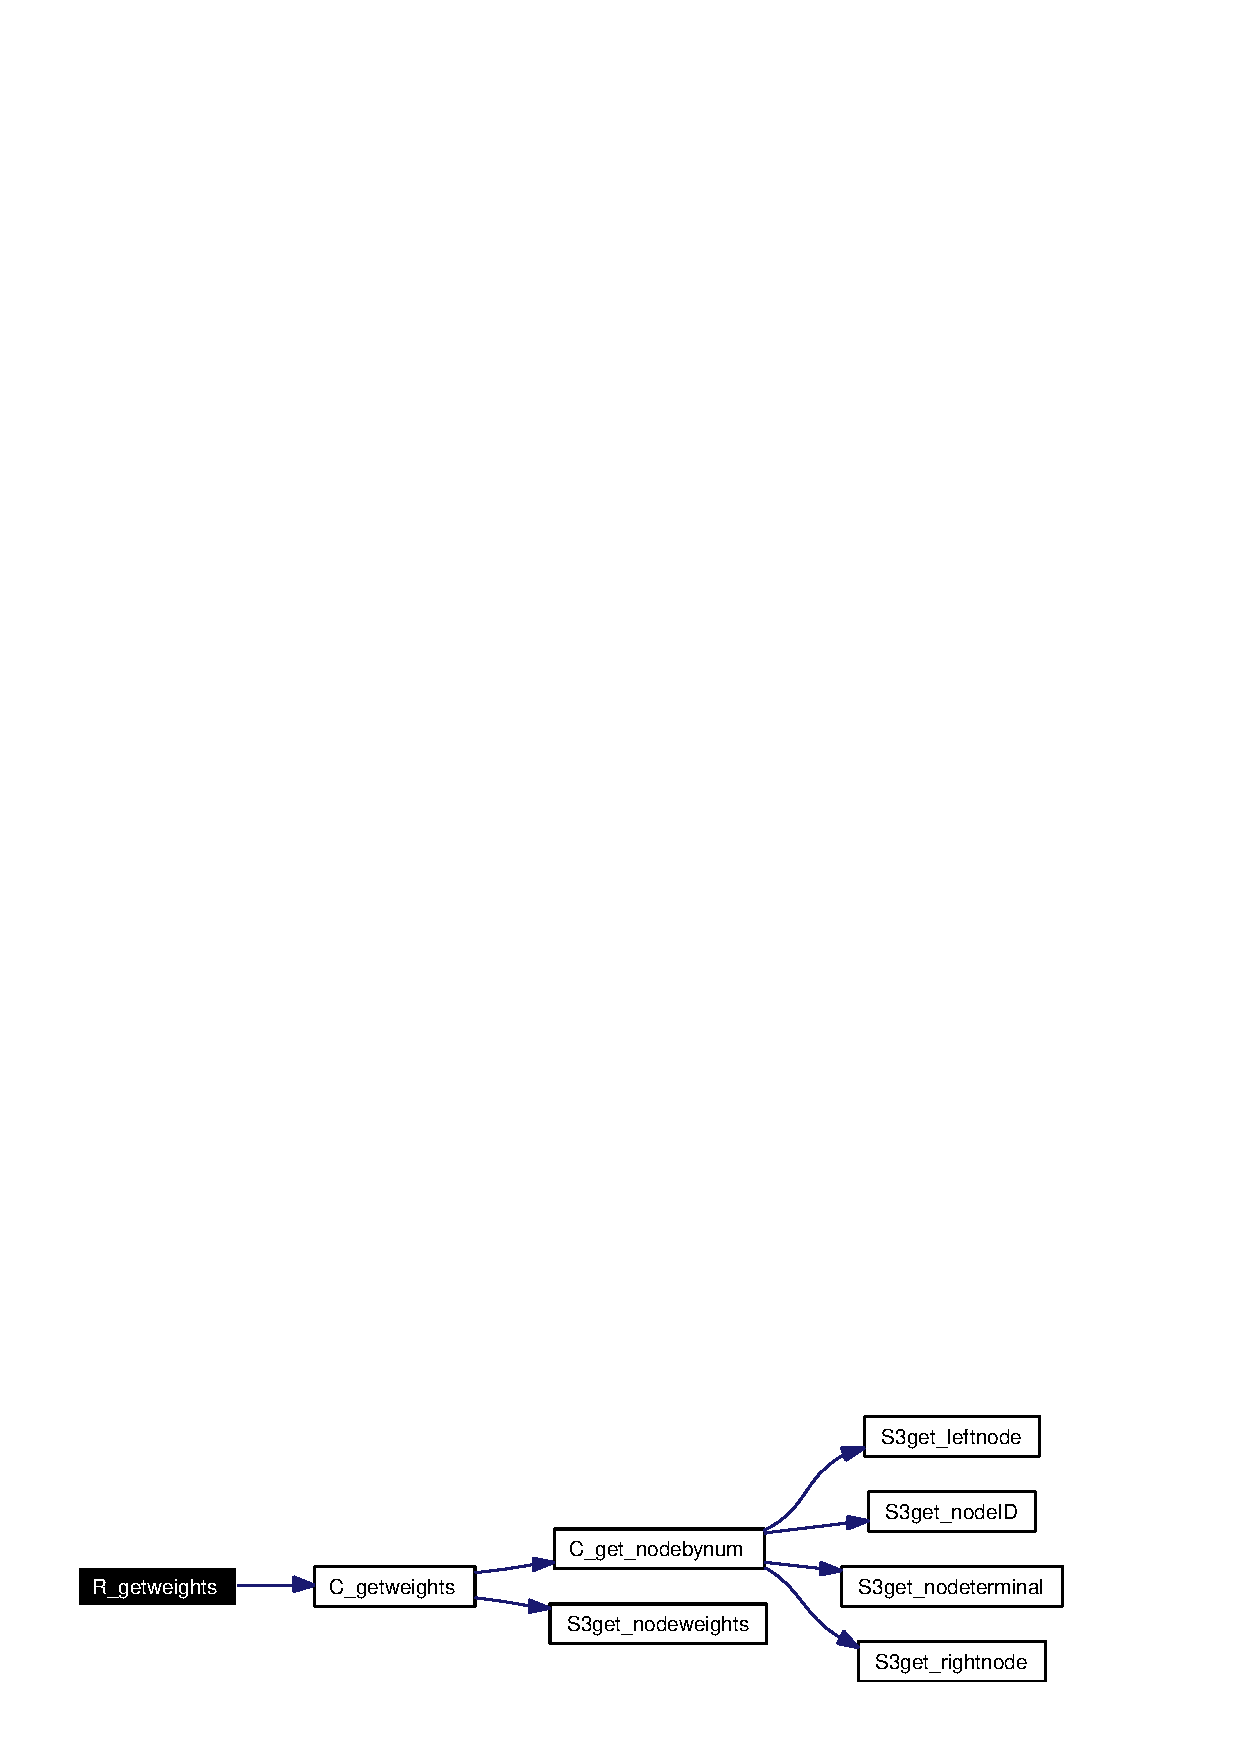
\includegraphics[width=262pt]{Predict_8c_a14_cgraph}
\end{center}
\end{figure}
\hypertarget{Predict_8c_a10}{
\index{Predict.c@{Predict.c}!R_predict@{R\_\-predict}}
\index{R_predict@{R\_\-predict}!Predict.c@{Predict.c}}
\subsubsection[R\_\-predict]{\setlength{\rightskip}{0pt plus 5cm}SEXP R\_\-predict (SEXP {\em tree}, SEXP {\em newinputs}, SEXP {\em mincriterion})}}
\label{Predict_8c_a10}


R-Interface to C\_\-predict \par
 \begin{Desc}
\item[Parameters:]
\begin{description}
\item[{\em tree}]a tree \item[{\em newinputs}]an object of class `Variable\-Frame' \item[{\em mincriterion}]overwrites mincriterion used for tree growing \end{description}
\end{Desc}


Definition at line 374 of file Predict.c.

References C\_\-predict(), and get\_\-nobs().

Here is the call graph for this function:\begin{figure}[H]
\begin{center}
\leavevmode
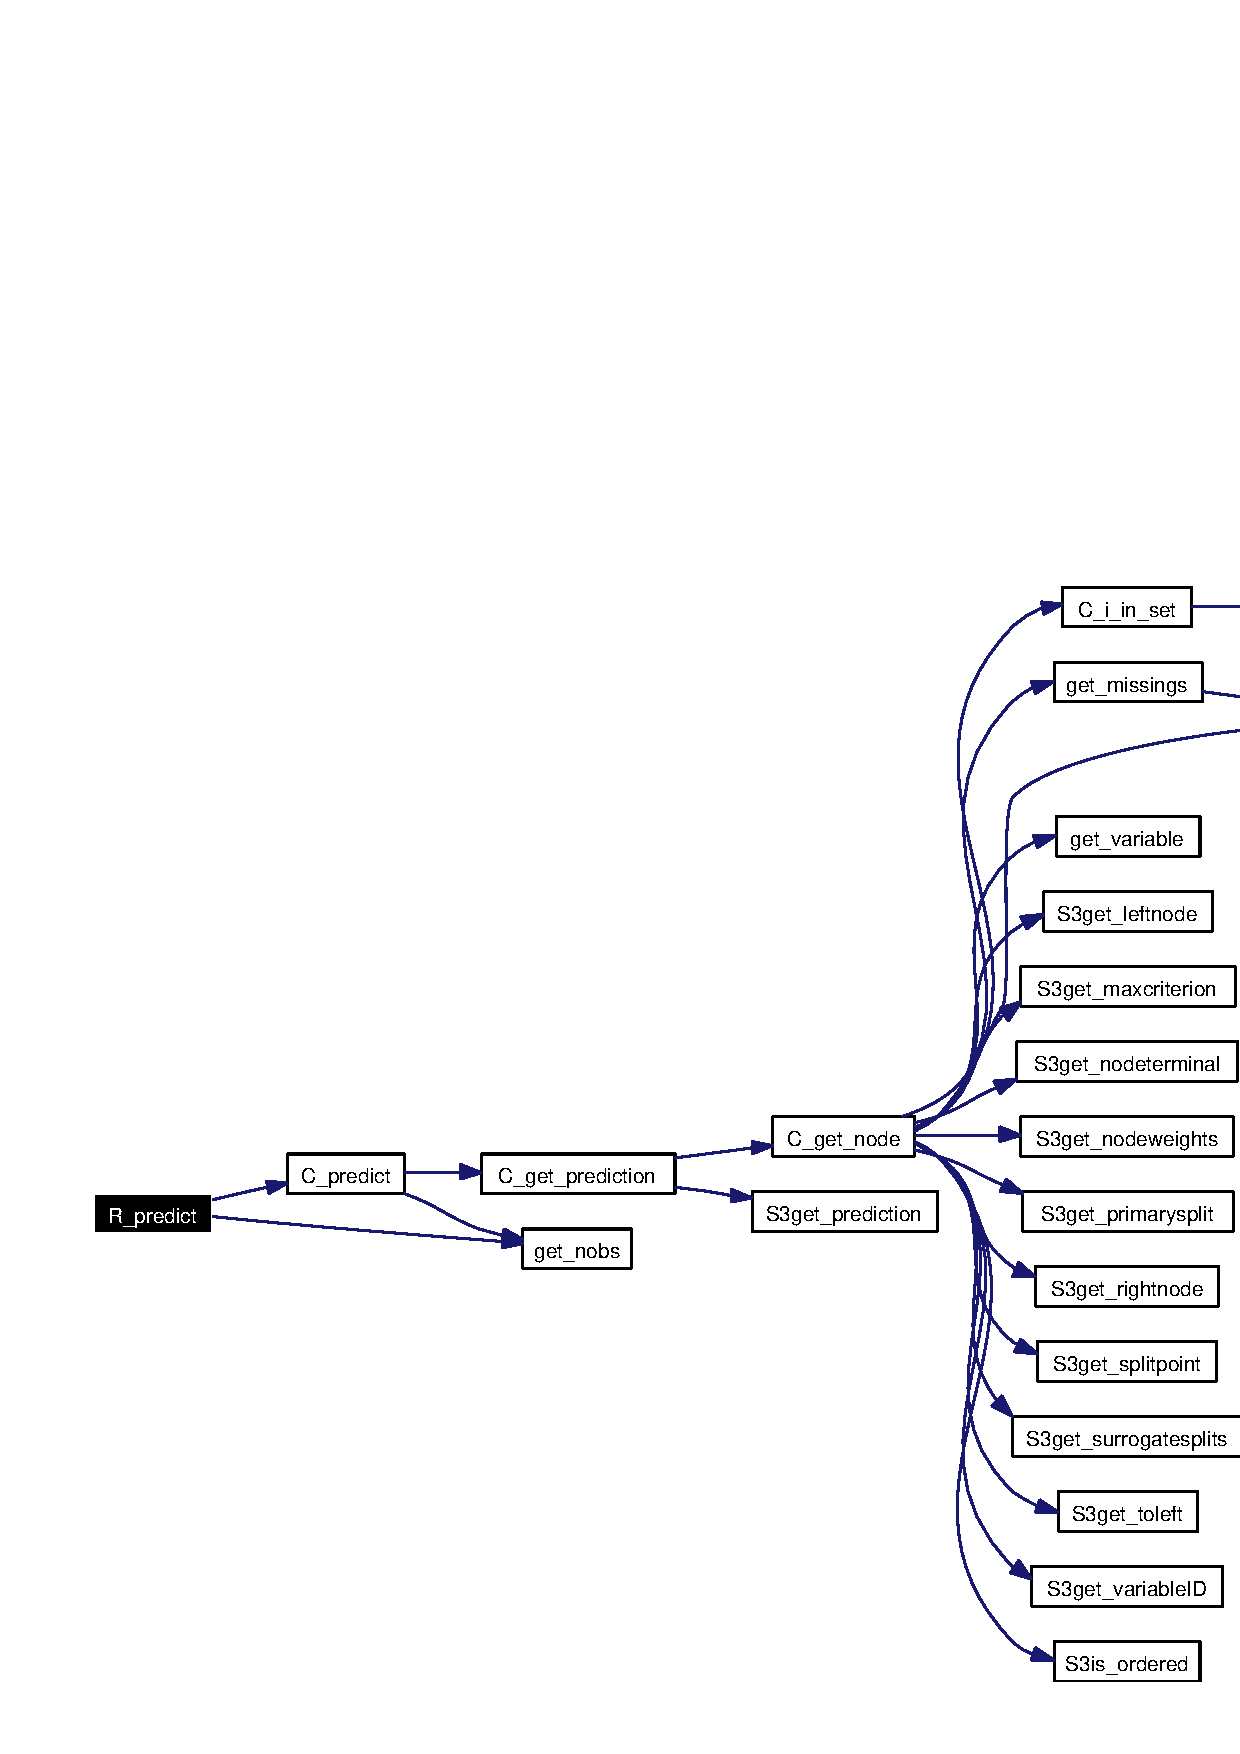
\includegraphics[width=356pt]{Predict_8c_a10_cgraph}
\end{center}
\end{figure}
\hypertarget{Predict_8c_a17}{
\index{Predict.c@{Predict.c}!R_predictRF@{R\_\-predictRF}}
\index{R_predictRF@{R\_\-predictRF}!Predict.c@{Predict.c}}
\subsubsection[R\_\-predictRF]{\setlength{\rightskip}{0pt plus 5cm}SEXP R\_\-predict\-RF (SEXP {\em forest}, SEXP {\em newinputs}, SEXP {\em mincriterion}, SEXP {\em oobpred})}}
\label{Predict_8c_a17}


Predictions from Random\-Forest objects \begin{Desc}
\item[Parameters:]
\begin{description}
\item[{\em forest}]a list of trees \item[{\em newinputs}]an object of class `Variable\-Frame' \item[{\em mincriterion}]overwrites mincriterion used for tree growing \item[{\em oobpred}]a logical indicating out-of-bag predictions \end{description}
\end{Desc}


Definition at line 520 of file Predict.c.

References C\_\-get\_\-nodebynum(), C\_\-get\_\-node\-ID(), get\_\-nobs(), S3get\_\-nodeweights(), and S3get\_\-prediction().

Here is the call graph for this function:\begin{figure}[H]
\begin{center}
\leavevmode
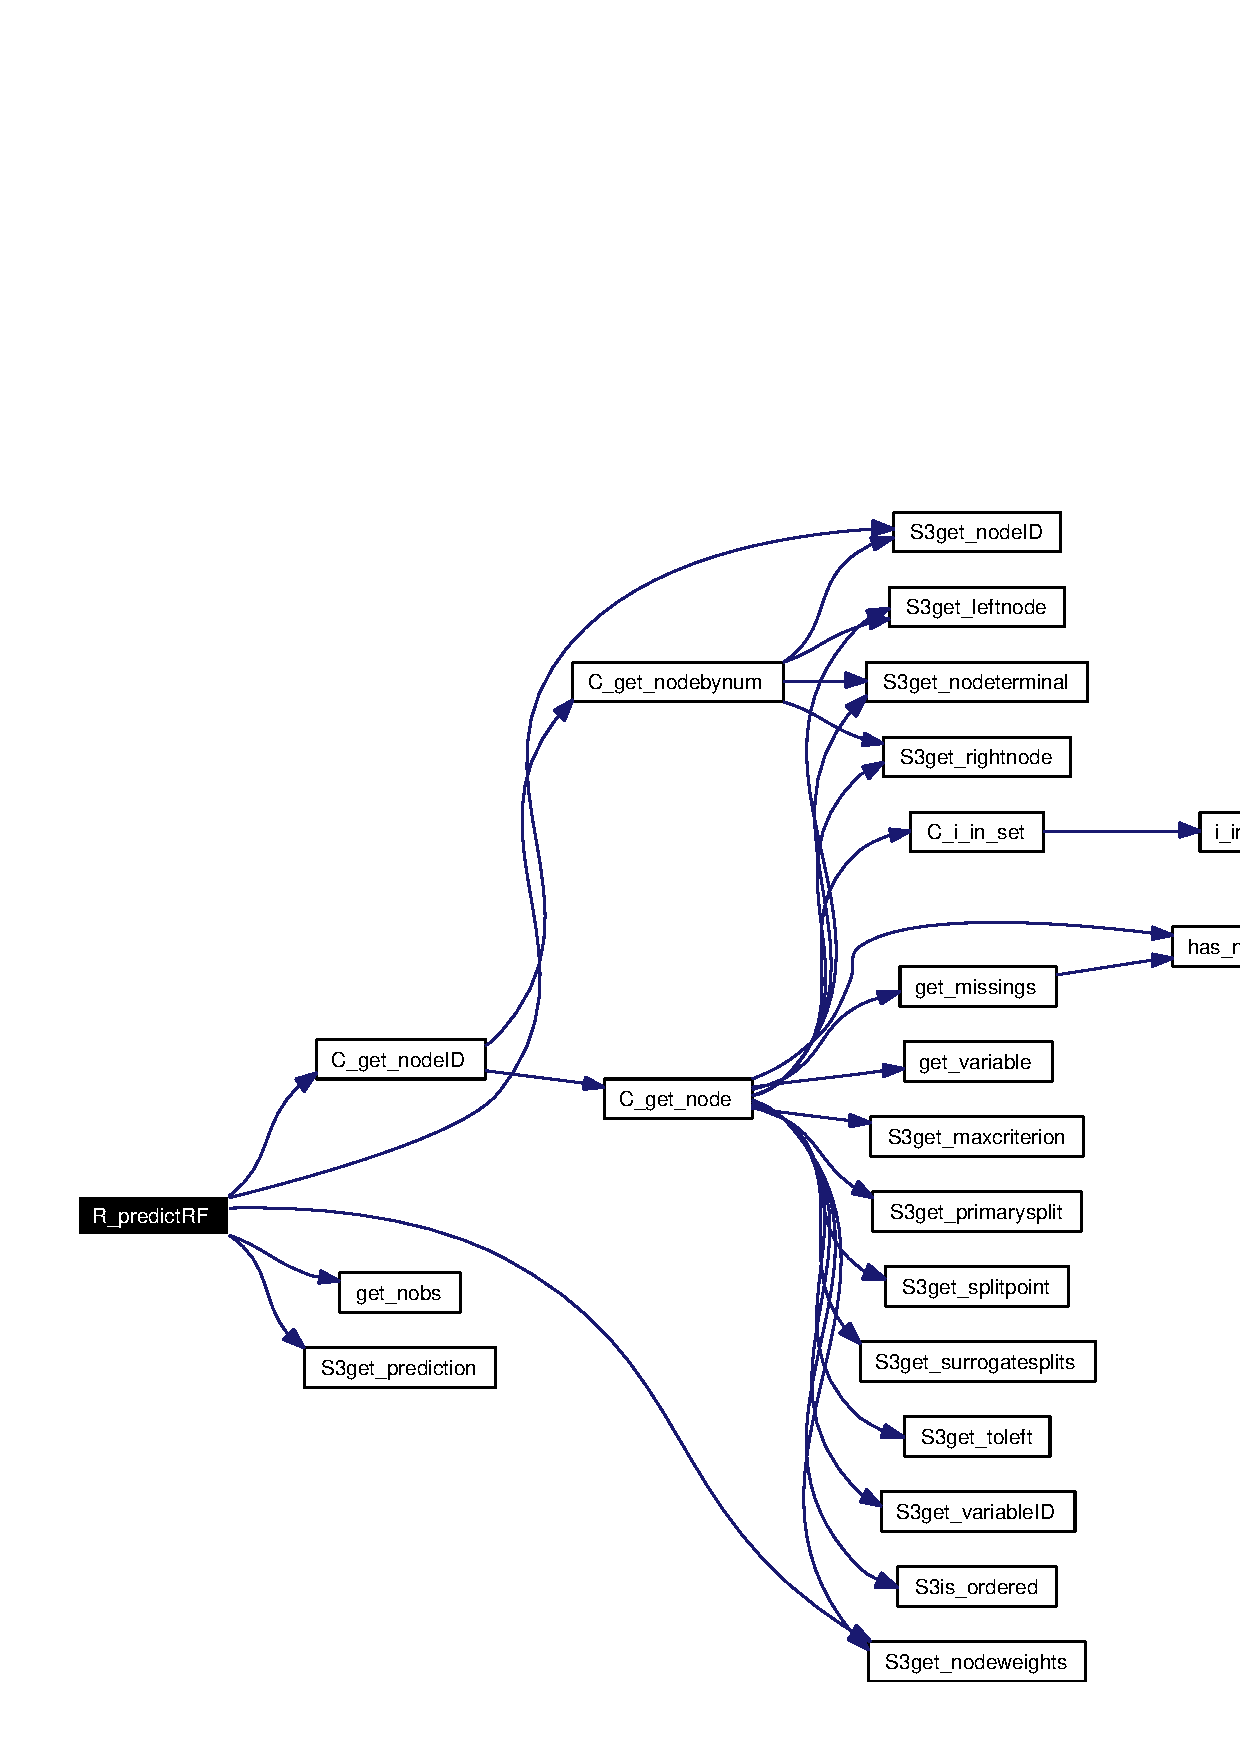
\includegraphics[width=324pt]{Predict_8c_a17_cgraph}
\end{center}
\end{figure}
\hypertarget{Predict_8c_a18}{
\index{Predict.c@{Predict.c}!R_predictRF2@{R\_\-predictRF2}}
\index{R_predictRF2@{R\_\-predictRF2}!Predict.c@{Predict.c}}
\subsubsection[R\_\-predictRF2]{\setlength{\rightskip}{0pt plus 5cm}SEXP R\_\-predict\-RF2 (SEXP {\em forest}, SEXP {\em response}, SEXP {\em newinputs}, SEXP {\em mincriterion}, SEXP {\em oobpred})}}
\label{Predict_8c_a18}


Predictions from Random\-Forest objects, based in total weights \begin{Desc}
\item[Parameters:]
\begin{description}
\item[{\em forest}]a list of trees \item[{\em response}]a matrix of (transformed) response values \item[{\em newinputs}]an object of class `Variable\-Frame' \item[{\em mincriterion}]overwrites mincriterion used for tree growing \item[{\em oobpred}]a logical indicating out-of-bag predictions \end{description}
\end{Desc}


Definition at line 576 of file Predict.c.

References C\_\-get\_\-nodebynum(), C\_\-get\_\-node\-ID(), C\_\-matprod(), get\_\-nobs(), ncol(), nrow(), and S3get\_\-nodeweights().

Here is the call graph for this function:\begin{figure}[H]
\begin{center}
\leavevmode
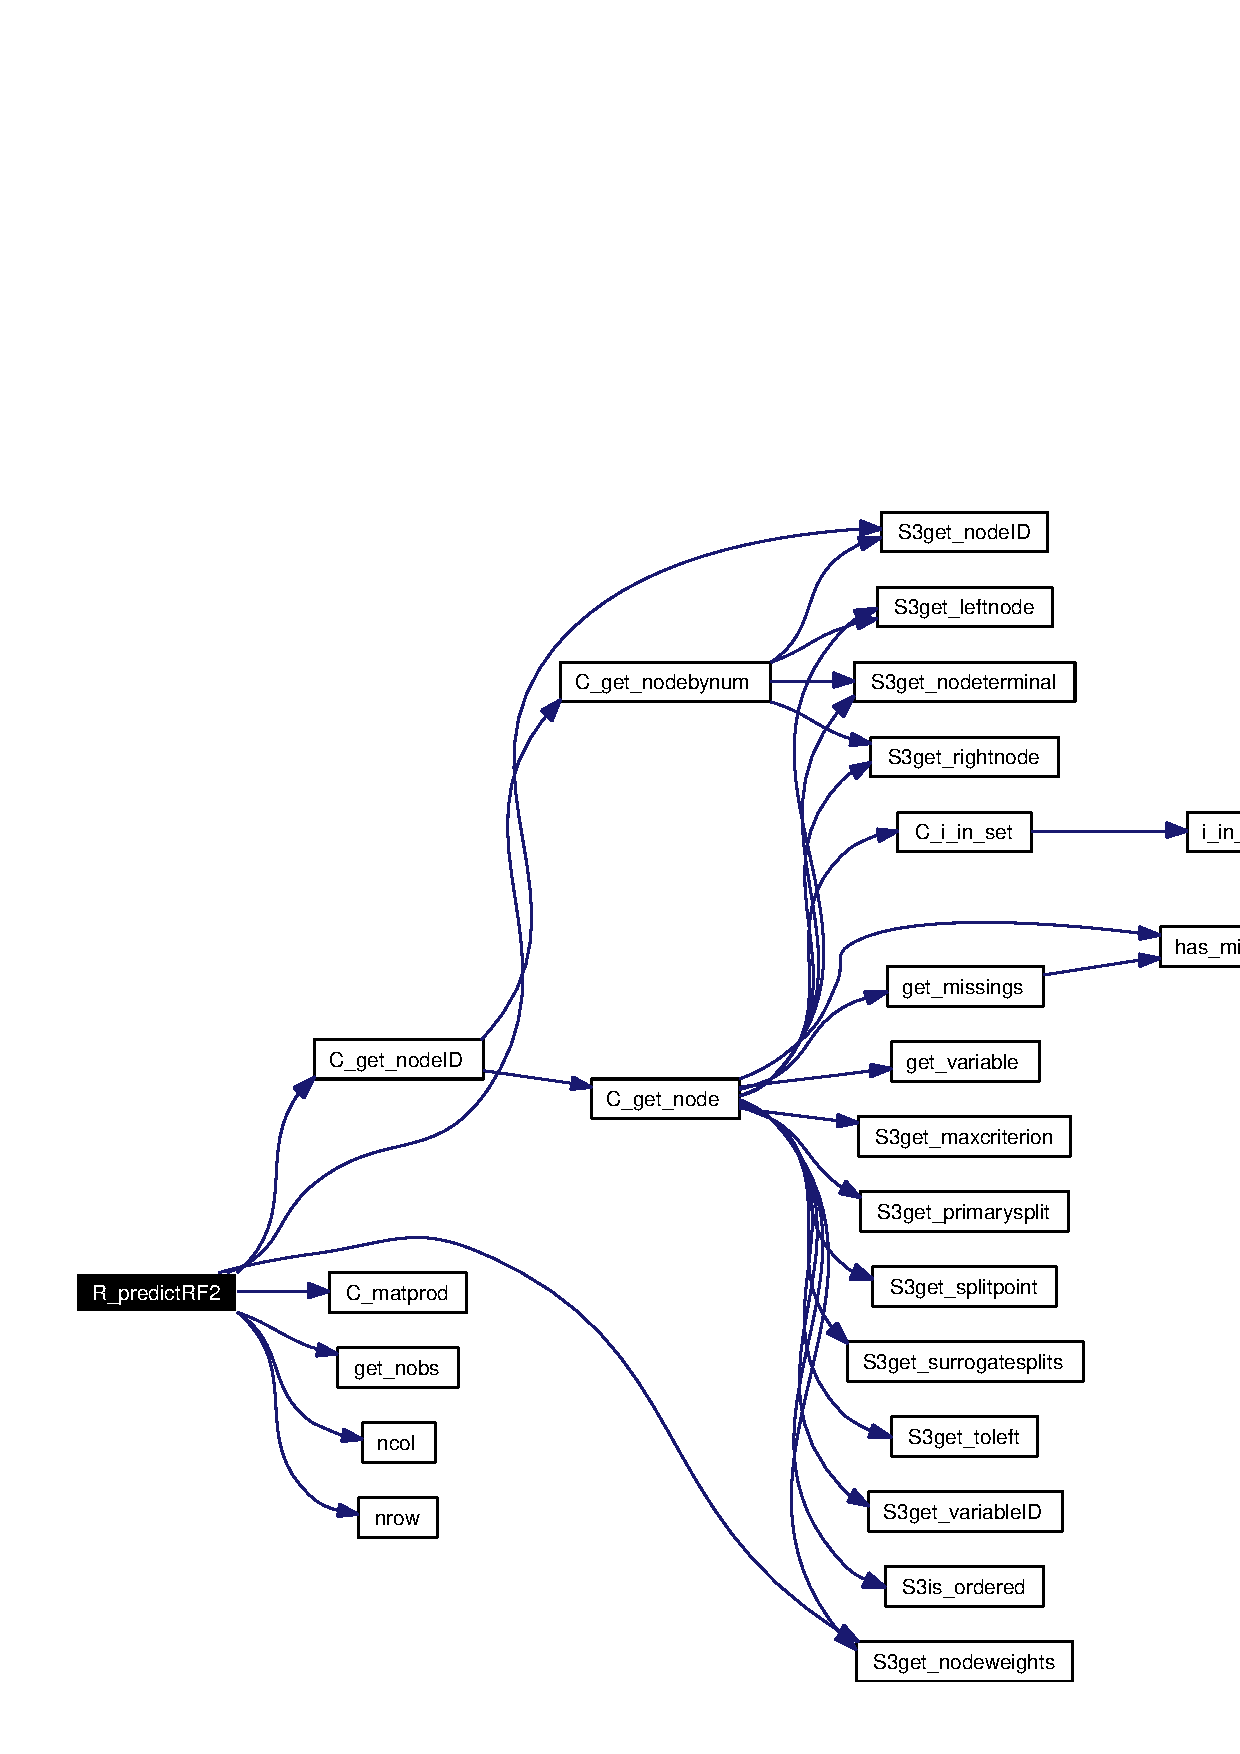
\includegraphics[width=322pt]{Predict_8c_a18_cgraph}
\end{center}
\end{figure}
\hypertarget{Predict_8c_a19}{
\index{Predict.c@{Predict.c}!R_predictRF_weights@{R\_\-predictRF\_\-weights}}
\index{R_predictRF_weights@{R\_\-predictRF\_\-weights}!Predict.c@{Predict.c}}
\subsubsection[R\_\-predictRF\_\-weights]{\setlength{\rightskip}{0pt plus 5cm}SEXP R\_\-predict\-RF\_\-weights (SEXP {\em forest}, SEXP {\em newinputs}, SEXP {\em mincriterion}, SEXP {\em oobpred})}}
\label{Predict_8c_a19}


Predictions weights from Random\-Forest objects \begin{Desc}
\item[Parameters:]
\begin{description}
\item[{\em forest}]a list of trees \item[{\em newinputs}]an object of class `Variable\-Frame' \item[{\em mincriterion}]overwrites mincriterion used for tree growing \item[{\em oobpred}]a logical indicating out-of-bag predictions \end{description}
\end{Desc}


Definition at line 641 of file Predict.c.

References C\_\-get\_\-nodebynum(), C\_\-get\_\-node\-ID(), get\_\-nobs(), S3get\_\-nodeweights(), and S3get\_\-prediction().

Here is the call graph for this function:\begin{figure}[H]
\begin{center}
\leavevmode
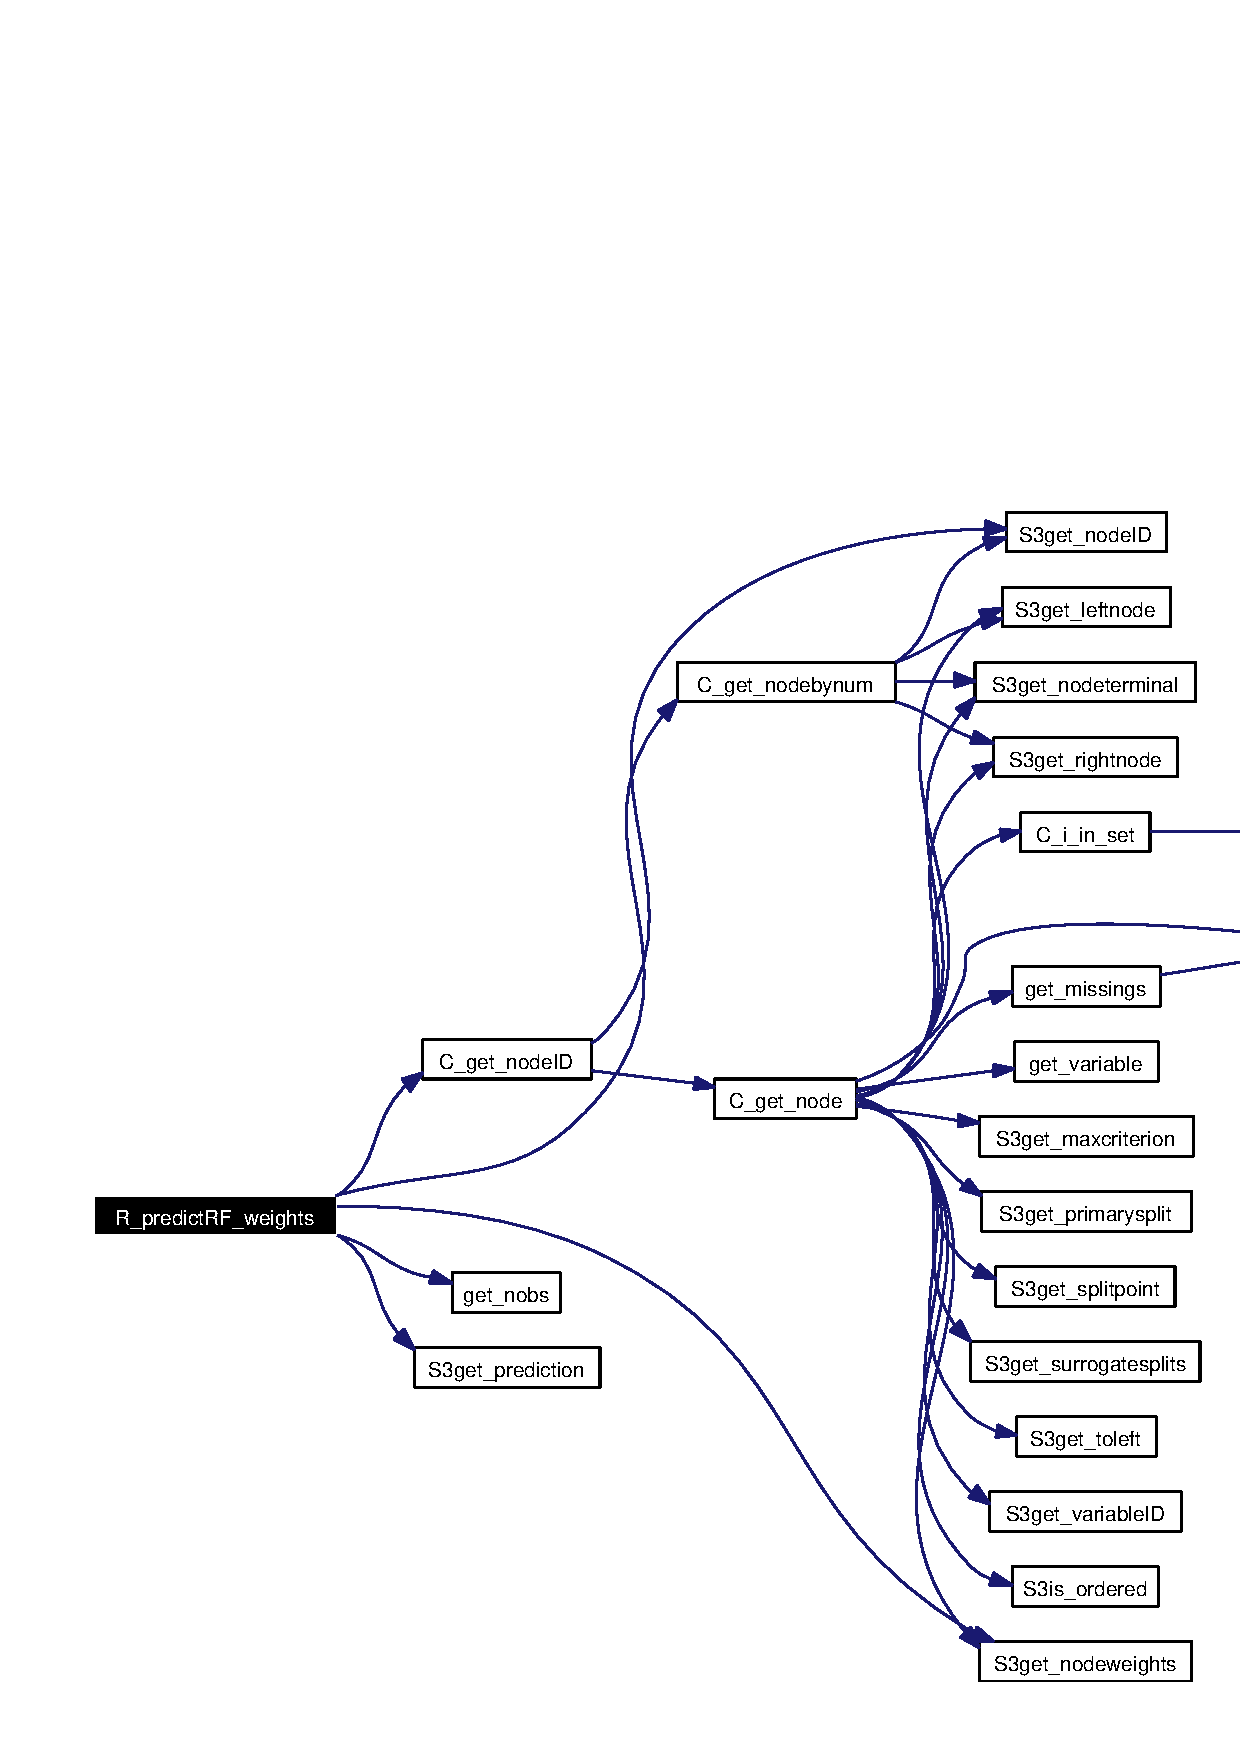
\includegraphics[width=346pt]{Predict_8c_a19_cgraph}
\end{center}
\end{figure}
\hypertarget{Predict_8c_a16}{
\index{Predict.c@{Predict.c}!R_weights@{R\_\-weights}}
\index{R_weights@{R\_\-weights}!Predict.c@{Predict.c}}
\subsubsection[R\_\-weights]{\setlength{\rightskip}{0pt plus 5cm}SEXP R\_\-weights (SEXP {\em tree}, SEXP {\em newinputs}, SEXP {\em mincriterion})}}
\label{Predict_8c_a16}


R-Interface to C\_\-weights \par
 \begin{Desc}
\item[Parameters:]
\begin{description}
\item[{\em tree}]a tree \item[{\em newinputs}]an object of class `Variable\-Frame' \item[{\em mincriterion}]overwrites mincriterion used for tree growing \end{description}
\end{Desc}


Definition at line 499 of file Predict.c.

References C\_\-weights(), and get\_\-nobs().

Here is the call graph for this function:\begin{figure}[H]
\begin{center}
\leavevmode
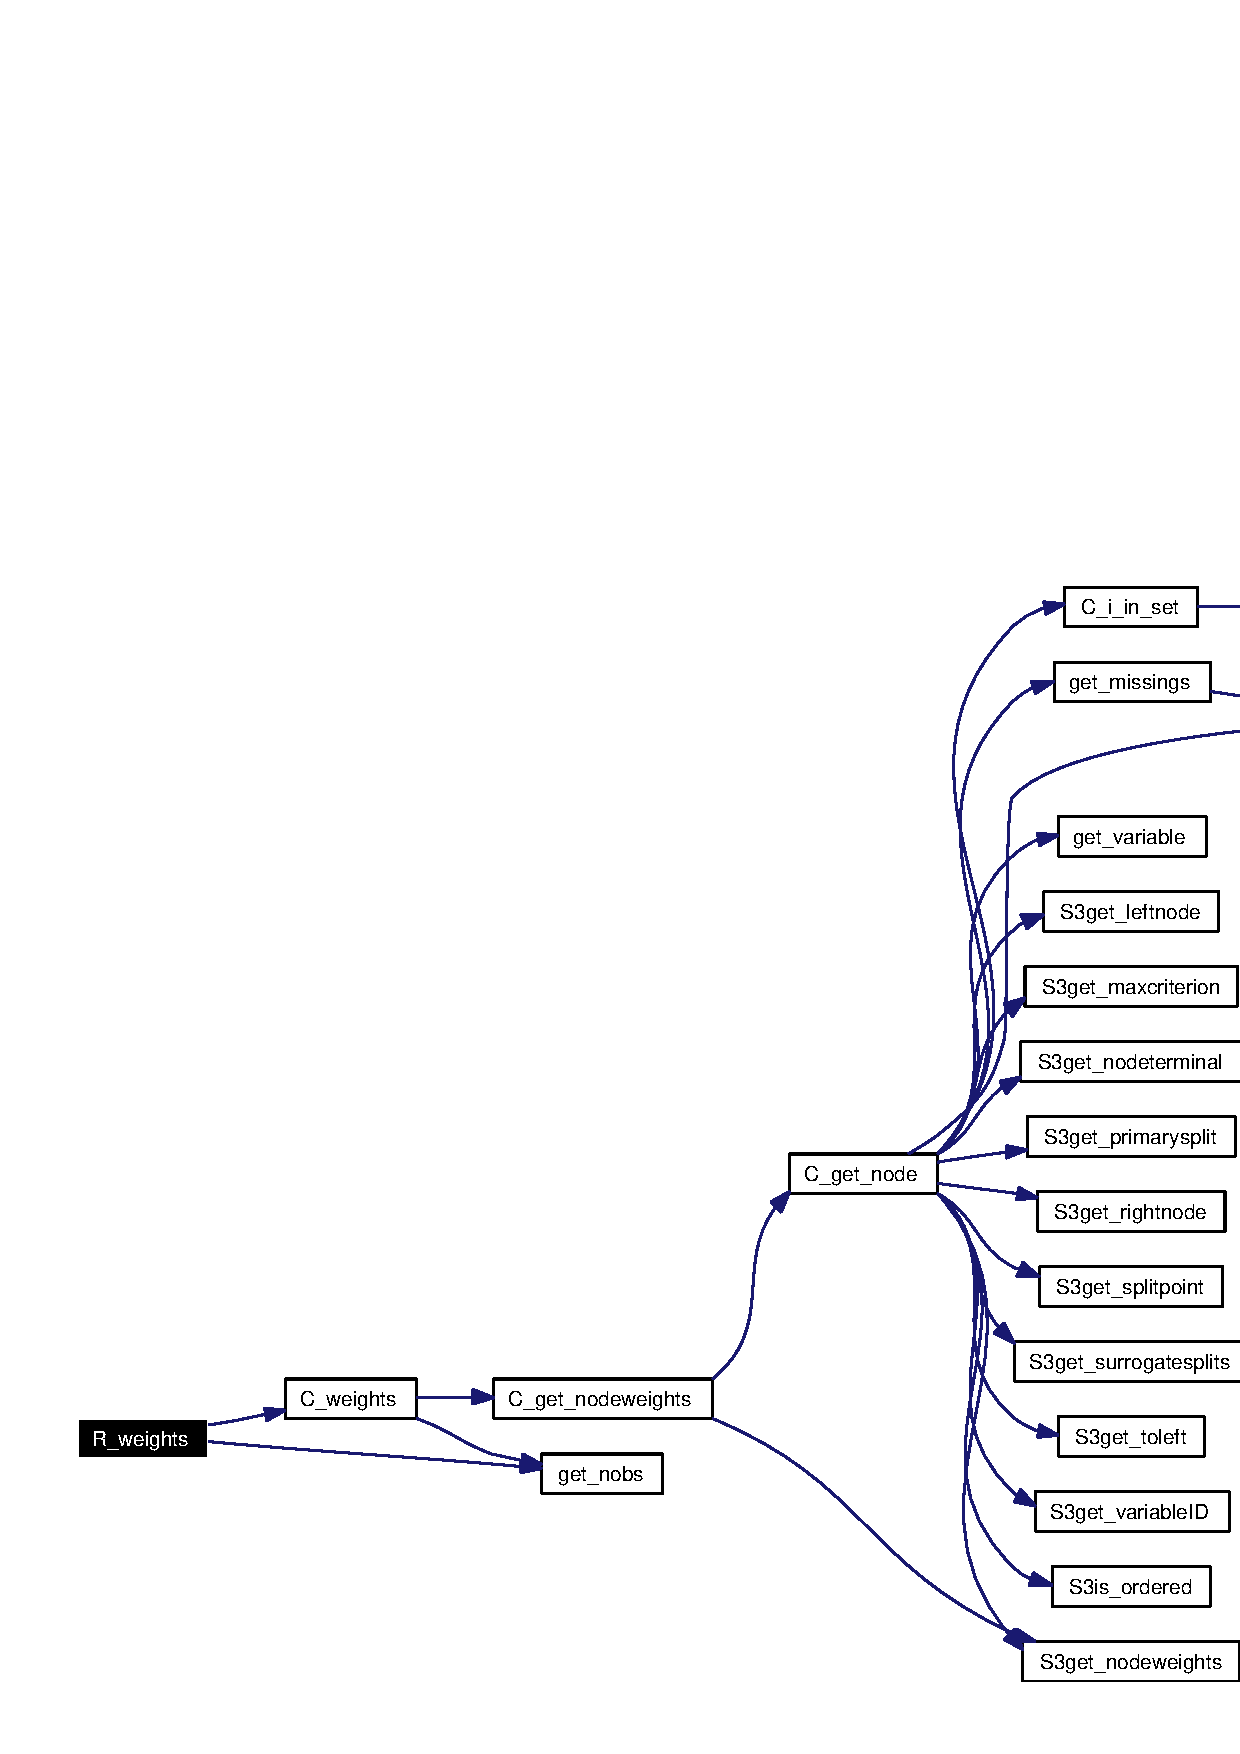
\includegraphics[width=355pt]{Predict_8c_a16_cgraph}
\end{center}
\end{figure}
